\documentclass[12pt,a4paper]{article}

% ── Codificación y lenguaje ──────────────────────────────────────────────────
\usepackage[T1]{fontenc}
\usepackage[utf8]{inputenc}
\usepackage[spanish,es-nodecimaldot]{babel}

% ── Geometría ────────────────────────────────────────────────────────────────
\usepackage[top=2.5cm,bottom=2.5cm,left=2.5cm,right=2.5cm,
            headheight=15pt]{geometry}

% ── Tipografía ───────────────────────────────────────────────────────────────
\usepackage{microtype}
\usepackage{lmodern}

% ── Matemáticas ──────────────────────────────────────────────────────────────
\usepackage{amsmath,amssymb}

% ── Color ────────────────────────────────────────────────────────────────────
\usepackage{xcolor}
\definecolor{azul}{RGB}{0,70,127}
\definecolor{azulclaro}{RGB}{31,73,125}
\definecolor{grisclaro}{RGB}{245,245,245}
\definecolor{verdeos}{RGB}{0,128,64}

% ── Encabezados y pie de página ───────────────────────────────────────────────
\usepackage{fancyhdr}
\usepackage{lastpage}
\pagestyle{fancy}
\fancyhf{}
\fancyhead[L]{\small\color{gray}Cálculo Vectorial — Motor de Gradiente}
\fancyhead[R]{\small\color{gray}Universidad de La Sabana}
\fancyfoot[C]{\small\thepage\ de \pageref{LastPage}}
\renewcommand{\headrulewidth}{0.4pt}

% ── Formato de secciones ─────────────────────────────────────────────────────
\usepackage{titlesec}
\titleformat{\section}{\large\bfseries\color{azul}}{\thesection.}{0.5em}{}
\titleformat{\subsection}{\normalsize\bfseries\color{azulclaro}}{\thesubsection.}{0.5em}{}
\titleformat{\subsubsection}{\normalsize\bfseries\color{azulclaro}}{\thesubsubsection.}{0.5em}{}

% ── Hyperref ──────────────────────────────────────────────────────────────────
\usepackage{hyperref}
\hypersetup{
  colorlinks=true, linkcolor=azul, urlcolor=azul, citecolor=azul,
  pdftitle={Movimiento lateral como flujo gradiente — Motor de Gradiente},
}

% ── Tablas ───────────────────────────────────────────────────────────────────
\usepackage{booktabs}
\usepackage{array}

% ── Figuras ──────────────────────────────────────────────────────────────────
\usepackage{graphicx}
\usepackage{caption}
\usepackage{subcaption}
\graphicspath{{imgs/}}
\captionsetup{font=small,labelfont=bf}

% ── Cajas destacadas ─────────────────────────────────────────────────────────
\usepackage{tcolorbox}
\tcbuselibrary{breakable,skins}
\tcbset{defbox/.style={enhanced,breakable,colback=grisclaro,colframe=azul,
  fonttitle=\bfseries,left=6pt,right=6pt,top=4pt,bottom=4pt}}

% ── Código fuente ─────────────────────────────────────────────────────────────
\usepackage{listings}
\lstset{
  basicstyle=\ttfamily\footnotesize,
  backgroundcolor=\color{grisclaro},
  frame=single,framerule=0.4pt,
  breaklines=true,numbers=left,numberstyle=\tiny\color{gray},
  keywordstyle=\color{azul}\bfseries,
  commentstyle=\color{gray}\itshape,
  stringstyle=\color{verdeos},
  language=Python,
  showstringspaces=false,
  xleftmargin=1.5em,
}

% ── Enumeraciones ─────────────────────────────────────────────────────────────
\usepackage{float}
\usepackage{enumitem}

% ── Comandos matemáticos ──────────────────────────────────────────────────────
\newcommand{\grad}{\nabla}
\newcommand{\norm}[1]{\left\|#1\right\|}

% ═════════════════════════════════════════════════════════════════════════════
\begin{document}
\thispagestyle{empty}

% ── Portada ───────────────────────────────────────────────────────────────────
\begin{center}
  Universidad de La Sabana\\
  Facultad de Ingeniería\\[4pt]
  \textbf{Taller de Cálculo Vectorial}
\end{center}
\noindent\rule{\linewidth}{0.8pt}
\begin{center}
  \vspace{6pt}
  {\LARGE\bfseries Movimiento lateral de un atacante\\[4pt]
  como flujo gradiente}\\[8pt]
  {\normalsize Una perspectiva vectorial de la ciberseguridad ofensiva\\
  con validación en laboratorio Wazuh\,+\,Suricata en tiempo real}
  \vspace{4pt}
\end{center}
\noindent\rule{\linewidth}{0.8pt}
\vspace{1.2cm}
\begin{center}
\begin{tabular}{rl}
  \textbf{Integrantes:}  & Daniel Pareja Franco \\
                         & Santiago José Curi \\
                         & Sebastián Páez \\
                         & Nicole Bonilla \\[6pt]
  \textbf{Asignatura:}   & Cálculo Vectorial \\[3pt]
  \textbf{Campo elegido:}& Ciberseguridad ofensiva --- movimiento lateral (MITRE TA0008) \\[3pt]
  \textbf{Herramienta computacional:} &
    Python 3.11 $\cdot$ NumPy $\cdot$ SciPy $\cdot$ Matplotlib $\cdot$ Wazuh 4.7.5 \\[3pt]
  \textbf{Infraestructura:} &
    DigitalOcean (3 VMs Ubuntu) $\cdot$ Kali Linux $\cdot$ Suricata IDS \\[3pt]
  \textbf{Fecha:} & Mayo de 2026
\end{tabular}
\end{center}
\vfill
\begin{tcolorbox}[defbox]
  \textbf{Declaración metodológica.}
  Este proyecto combina un modelo analítico cerrado~(Fase~1) con un
  laboratorio real en la nube~(Fase~2). En la Fase~1, $V(x,y)$ se
  construye de forma explícita y todos los resultados son exactos.
  En la Fase~2, $V$ se alimenta de alertas reales de Wazuh y Suricata,
  haciendo que el campo escalar evolucione en tiempo real durante el
  ataque simulado. Todos los scripts, configuraciones y datos del
  experimento están disponibles en el repositorio del proyecto.
\end{tcolorbox}

\newpage
\tableofcontents
\newpage

% ═════════════════════════════════════════════════════════════════════════════
\section{Planteamiento del problema}

En un ataque informático dirigido, el adversario rara vez compromete
directamente su objetivo final. Primero obtiene acceso a un nodo de
baja seguridad y luego se \textbf{mueve lateralmente} por la red
saltando de equipo en equipo hasta alcanzar el activo de mayor valor:
una base de datos, un servidor de control o credenciales administrativas.
Este proceso no es aleatorio: un atacante con información sobre la red
elige en cada paso el nodo que maximiza su acceso futuro con el menor
riesgo de detección. Esa toma de decisiones tiene una estructura
matemática precisa.

\begin{tcolorbox}[defbox, title=Pregunta central del proyecto]
  ¿Puede el gradiente de un campo escalar de vulnerabilidad modelar
  la trayectoria óptima de un atacante en movimiento lateral, y qué
  revela ese modelo sobre dónde concentrar las defensas?
\end{tcolorbox}

% ═════════════════════════════════════════════════════════════════════════════
\section{Infraestructura del laboratorio}

\subsection{Wazuh SIEM}

\textbf{Wazuh} es una plataforma de código abierto para \emph{Security
Information and Event Management} (SIEM). Recopila, normaliza y
correlaciona eventos de seguridad de múltiples fuentes en tiempo real.

\medskip
La arquitectura consta de tres componentes principales:

\begin{itemize}
  \item \textbf{Agentes}: procesos ligeros instalados en cada host
    monitorizado. Recolectan logs del sistema operativo (syslog, auth.log,
    dpkg), ejecutan comprobaciones de integridad de archivos (FIM) y envían
    todo al manager vía canal cifrado.
  \item \textbf{Manager}: servidor central que recibe los eventos de los
    agentes, aplica el motor de reglas y genera las alertas. Las alertas
    se almacenan en \texttt{/var/ossec/logs/alerts/alerts.json} como
    objetos JSON, uno por línea.
  \item \textbf{Dashboard}: interfaz web que consume el índice de alertas
    almacenado en OpenSearch (heredero de Elasticsearch).
\end{itemize}

Cada alerta generada por Wazuh incluye, entre otros campos:

\begin{table}[H]
  \centering
  \caption{Campos relevantes de una alerta Wazuh (extracto del JSON).}
  \begin{tabular}{@{}lll@{}}
    \toprule
    Campo & Tipo & Descripción \\
    \midrule
    \texttt{timestamp}       & string ISO 8601 & Momento del evento \\
    \texttt{agent.id}        & string (3 dígitos) & Identificador del agente origen \\
    \texttt{agent.name}      & string & Hostname del agente \\
    \texttt{rule.id}         & entero & ID de la regla que disparó la alerta \\
    \texttt{rule.level}      & entero (1--15) & Severidad: $\leq 4$ info, 5--7 bajo, 8--10 alto, $\geq 11$ crítico \\
    \texttt{rule.description}& string & Descripción legible de la alerta \\
    \texttt{rule.mitre.tactic} & lista & Táctica(s) MITRE ATT\&CK asociada(s) \\
    \texttt{rule.mitre.id}   & lista & Técnica(s) MITRE (e.g.\ T1110.001) \\
    \bottomrule
  \end{tabular}
\end{table}

\begin{tcolorbox}[defbox]
  \textbf{Nota técnica.} Wazuh 4.7.5 no expone un endpoint REST
  \texttt{/alerts} (fue eliminado en versiones post-4.3). El motor de
  gradiente accede a las alertas directamente vía SSH leyendo
  \texttt{alerts.json} con \texttt{tail -n 5000}, filtrando por
  \texttt{agent.id} y ventana temporal.
\end{tcolorbox}

\subsection{Suricata IDS}

\textbf{Suricata} es un motor de detección de intrusiones de red
(\emph{Network IDS/IPS}) de código abierto. Analiza el tráfico de red
a nivel de paquete y dispara alertas cuando detecta patrones maliciosos
definidos en sus reglas.

En el laboratorio, Suricata corre en el manager y monitoriza el tráfico
entrante hacia los nodos víctima. Las reglas provienen del conjunto
\textbf{Emerging Threats} (ET), que incluye:

\begin{itemize}
  \item \textbf{ET DROP}: bloqueo de IPs en listas negras (Dshield, CINS).
    Rule ID 86601.
  \item \textbf{ET CINS}: IPs con reputación baja según
    \emph{Active Threat Intelligence}. Rule ID 86601.
  \item \textbf{Alertas de autenticación SSH}: detectadas por el agente
    Wazuh a través del decoder de \texttt{sshd}. Rule ID 5710
    (\emph{sshd: Attempt to login using a non-existent user}),
    clasificadas como T1110.001 (Brute Force: Password Guessing) +
    T1021.004 (Remote Services: SSH) en el marco MITRE ATT\&CK.
\end{itemize}

\subsection{Estructura de alertas y datos extraídos}

El motor extrae únicamente alertas de \texttt{rule.level} $\geq 5$
para filtrar ruido operacional (heartbeats, syscollector, etc.). A
partir de esas alertas calcula el score de vulnerabilidad de cada nodo
con una fórmula de decaimiento temporal exponencial (véase
sección~\ref{sec:modelo}).

\subsection{Topología del laboratorio}

Tres máquinas virtuales Ubuntu en DigitalOcean actúan como nodos de
la red simulada. El atacante opera desde Kali Linux en red local
accediendo a los nodos por IP pública.

\begin{table}[H]
  \centering
  \caption{Nodos del laboratorio y su rol en el experimento.}
  \begin{tabular}{@{}lllcc@{}}
    \toprule
    Rol & Hostname & IP pública & Wazuh Agent ID & Pos.\ lógica \\
    \midrule
    Nodo A (entry)       & wazuh-manager        & 165.227.109.227 & 000 (manager) & $(0.5,0.5)$ \\
    Nodo B (víctima)     & victim-c             & 165.227.122.79  & 003           & $(3.0,3.0)$ \\
    Nodo C (crown jewel) & capstone-campusshield& 198.199.71.219  & 001           & $(7.0,3.0)$ \\
    Atacante             & Kali Linux           & 192.168.50.21   & ---           & --- \\
    \bottomrule
  \end{tabular}
\end{table}

\begin{figure}[H]
  \centering
  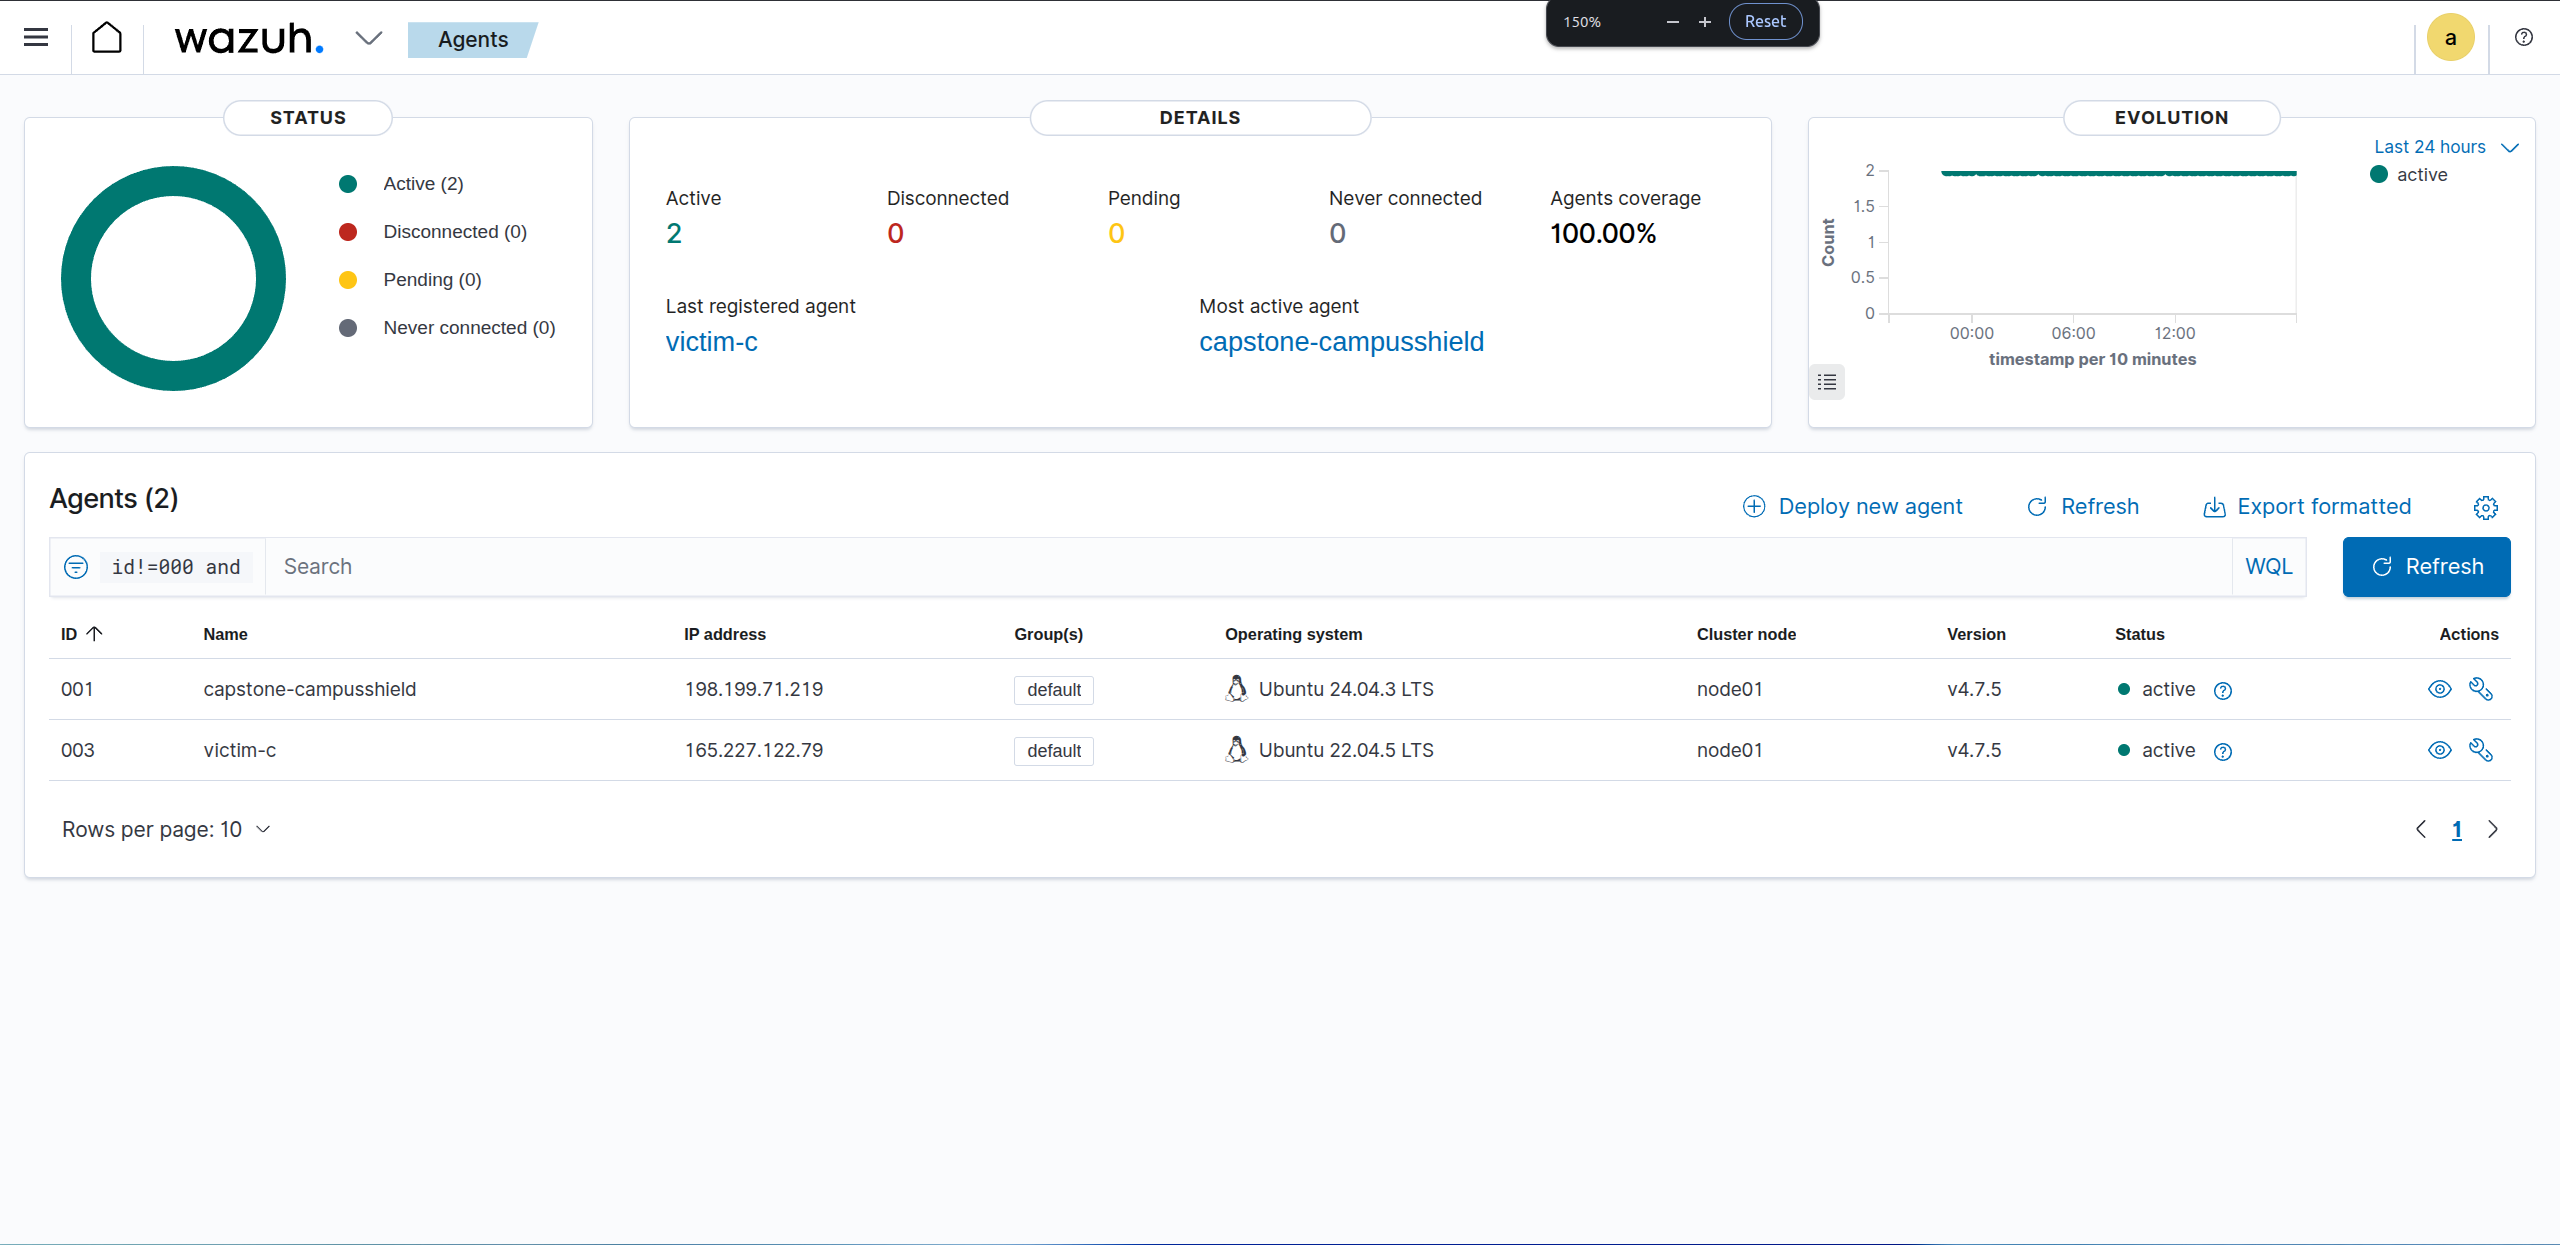
\includegraphics[width=0.7\linewidth]{wazuh_agents}
  \caption{Vista de agentes en el dashboard de Wazuh. Los dos agentes
    activos son capstone-campusshield~(001) y victim-c~(003), ambos
    ejecutando Wazuh v4.7.5. La cobertura es del 100\,\%.}
  \label{fig:wazuh_agents}
\end{figure}

% ═════════════════════════════════════════════════════════════════════════════
\section{Motor de gradiente en Python}

\subsection{Arquitectura del sistema}

El motor está compuesto por cinco módulos Python que se comunican a
través de la función principal en \texttt{main.py}. El flujo de datos
en cada iteración es:

\begin{center}
\textbf{Wazuh (SSH)} $\;\to\;$
\textbf{wazuh\_client} $\;\to\;$
\textbf{scalar\_field} $\;\to\;$
\textbf{gradient\_flow} $\;\to\;$
\textbf{visualizer}
\end{center}

Cada iteración dura aproximadamente 5 segundos (\texttt{POLL\_INTERVAL}).
Al finalizar, la figura generada se guarda en \texttt{/tmp/} y se
transfiere automáticamente vía SCP a la máquina local del analista.

\subsection{Módulo \texttt{wazuh\_client.py} — Adquisición y puntuación}

Este módulo reemplaza la comunicación REST de Wazuh con acceso directo
vía SSH al archivo de alertas. Contiene dos funciones principales:

\begin{lstlisting}[caption={Lectura de alertas vía SSH y filtrado temporal.}]
def get_alerts_for_agent(url, token, agent_id, last_n_minutes=3):
    since = datetime.now(timezone.utc) - timedelta(minutes=last_n_minutes)
    # Conexion SSH al manager y lectura de las ultimas 5000 lineas
    result = subprocess.run(
        ["ssh", "-o", "BatchMode=yes", f"root@165.227.109.227",
         "tail -n 5000 /var/ossec/logs/alerts/alerts.json"],
        capture_output=True, text=True, timeout=12)
    # Filtrar por agente y ventana temporal
    for line in result.stdout.splitlines():
        alert = json.loads(line)
        if alert["agent"]["id"].zfill(3) != agent_id.zfill(3): continue
        if datetime.fromisoformat(alert["timestamp"]) < since: continue
        alerts.append(alert)
    return alerts
\end{lstlisting}

\begin{lstlisting}[caption={Cálculo del score con decaimiento temporal y normalización logarítmica.}]
def score_from_alerts(alerts, decay_lambda=0.1):
    # Solo alertas nivel >= 5 (descartar ruido operacional)
    for alert in alerts:
        level = alert["rule"]["level"]
        if level < 5: continue
        delta_min = (now - ts).total_seconds() / 60
        # Peso: nivel de alerta * factor de decaimiento exponencial
        total += level * exp(-decay_lambda * delta_min)
    # Normalizacion log1p para evitar saturacion con muchas alertas
    score = log1p(total) / log1p(50) * 10.0
    return min(score, 10.0)
\end{lstlisting}

La normalización $\ln(1+x)/\ln(51)$ hace que el score crezca
rápidamente al inicio pero se aplane con volúmenes muy altos de
alertas, evitando que todos los nodos queden saturados en 10.0.

\subsection{Módulo \texttt{scalar\_field.py} — Campo escalar dinámico}

Construye $V(\mathbf{x}, t)$ como superposición de gaussianas centradas
en los nodos, con amplitudes iguales a los scores actuales. El parámetro
$\sigma = 1.5$ define el \textbf{radio de influencia} de cada nodo en
unidades lógicas: a distancia $\sigma$ del nodo, la contribución
gaussiana cae a $e^{-0.5} \approx 60\%$ del máximo; a distancia
$2\sigma$ cae a $e^{-2} \approx 14\%$. Un $\sigma$ más grande
«ensancha» los picos y suaviza el campo; uno más pequeño crea picos
más estrechos con gradientes más abruptos.

\begin{lstlisting}[caption={Construcción del campo escalar por superposición gaussiana.}]
def build_scalar_field(node_positions, scores, sigma, grid_size=200):
    X, Y = np.meshgrid(np.linspace(-2, 10, grid_size),
                       np.linspace(-2,  7, grid_size))
    V = np.zeros_like(X)
    for (px, py), s in zip(node_positions, scores):
        dist2 = (X - px)**2 + (Y - py)**2
        V += s * np.exp(-dist2 / (2 * sigma**2))
    return X, Y, V

def compute_gradient(X, Y, V):
    # Gradiente numerico con diferencias finitas (numpy.gradient)
    dVdy, dVdx = np.gradient(V, Y[:,0], X[0,:])
    return dVdx, dVdy

def find_critical_points(X, Y, dVdx, dVdy, threshold=0.02):
    # Puntos donde |gradiente| < umbral -> candidatos a puntos criticos
    mag = np.sqrt(dVdx**2 + dVdy**2)
    mask = mag < threshold
    # Agrupar puntos adyacentes con label de scipy
    ...
\end{lstlisting}

\subsection{Módulo \texttt{gradient\_flow.py} — Trayectoria y integral}

\begin{tcolorbox}[defbox]
  \textbf{¿Por qué dos etapas de integración?} El flujo gradiente
  $\mathbf{r}'(t) = \grad V(\mathbf{r}(t))$ converge siempre hacia el
  \emph{máximo local más cercano} al punto de partida. Cuando victim-c
  (B) y capstone (C) están ambos activos, B actúa como cuenca de
  atracción para puntos que parten desde el área de A. La trayectoria
  se «detiene» en B porque $\grad V \approx \mathbf{0}$ en un máximo.
  Para modelar el salto B$\to$C, se reinicia la integración desde el
  último punto de la etapa anterior, replicando la decisión del atacante
  de moverse al siguiente objetivo una vez comprometido B.
\end{tcolorbox}

Integra la EDO $\mathbf{r}'(t) = \grad V(\mathbf{r}(t))$ con el
solver RK45 de SciPy, que adapta el paso de integración automáticamente:

\begin{lstlisting}[caption={Integración numérica del flujo gradiente con RK45.}]
def integrate_attacker_path(X, Y, dVdx, dVdy, start, t_span, n_steps):
    # Interpolacion bilineal del gradiente en puntos arbitrarios
    interp_x = RegularGridInterpolator((Y[:,0], X[0,:]), dVdx)
    interp_y = RegularGridInterpolator((Y[:,0], X[0,:]), dVdy)

    def rhs(t, r):  # Lado derecho de la EDO
        return [interp_x([r[1], r[0]])[0],
                interp_y([r[1], r[0]])[0]]

    sol = solve_ivp(rhs, t_span, start, method='RK45',
                    t_eval=np.linspace(*t_span, n_steps))
    return np.array([sol.y[0], sol.y[1]])  # path[0]=x, path[1]=y

def compute_line_integral(X, Y, V, path):
    # TF de integrales de linea: V(destino) - V(origen)
    interp_V = RegularGridInterpolator((Y[:,0], X[0,:]), V)
    v_end   = interp_V([[path[1,-1], path[0,-1]]])[0]
    v_start = interp_V([[path[1, 0], path[0, 0]]])[0]
    return float(v_end - v_start)
\end{lstlisting}

\subsection{Módulo \texttt{visualizer.py} — Figura de cuatro paneles}

Genera en cada iteración una figura Matplotlib con fondo oscuro
compuesta por cuatro paneles:

\begin{enumerate}
  \item \textbf{Campo escalar $V(\mathbf{x})$}: mapa de calor con
    isolíneas. Las zonas más rojas corresponden a nodos con mayor
    actividad de alertas.
  \item \textbf{Gradiente $\grad V$}: campo vectorial quiver sobre
    el heatmap semitransparente. Las flechas cyan apuntan hacia los
    máximos del campo.
  \item \textbf{Trayectoria $\mathbf{r}(t)$}: integración en dos
    etapas — línea azul sólida~(A$\to$B) y naranja punteada~(B$\to$C).
    Marcadores: círculo verde (entrada), triángulo amarillo (pivote B),
    estrella roja (destino C).
  \item \textbf{Panel numérico}: iteración actual, integral de línea,
    número de puntos críticos y scores por nodo.
\end{enumerate}

\subsection{Loop principal: \texttt{main.py}}

El loop principal ejecuta en cada iteración:

\begin{enumerate}
  \item Consulta las alertas de los tres agentes vía SSH
  \item Calcula los scores con decaimiento temporal
  \item Construye $V(x,y)$ y calcula $\grad V$ numéricamente
  \item Integra la trayectoria en dos etapas (A$\to$B y B$\to$C)
  \item Calcula la integral de línea y detecta puntos críticos
  \item Actualiza la figura en pantalla y la guarda en \texttt{/tmp/}
  \item Transfiere la figura vía SCP al equipo local del analista
\end{enumerate}

Lo que se espera del motor: a medida que el simulador de ataque genera
alertas SSH en los nodos víctima, los picos gaussianos de $V$ deben
crecer, el gradiente debe orientarse hacia esos picos, y la trayectoria
$\mathbf{r}(t)$ debe mostrar el camino A$\to$B$\to$C de forma progresiva.

% ═════════════════════════════════════════════════════════════════════════════
\section{Conceptos de cálculo vectorial utilizados}

\begin{table}[H]
  \centering
  \caption{Conceptos del curso y su rol en el modelo.}
  \begin{tabular}{@{}p{5.5cm}p{8.5cm}@{}}
    \toprule
    Concepto & Rol en el modelo \\
    \midrule
    Campo escalar $V(\mathbf{x})$
      & Función de vulnerabilidad definida sobre el espacio lógico de la red \\
    Gradiente $\grad V$
      & Dirección de mayor vulnerabilidad en cada punto --- guía el ataque \\
    Curva parametrizada $\mathbf{r}(t)$
      & Trayectoria del atacante como solución de la EDO $\mathbf{r}'=\grad V$ \\
    Integral de línea $\int_C \grad V\cdot d\mathbf{r}$
      & Vulnerabilidad acumulada a lo largo del recorrido \\
    Campo conservativo
      & $\grad V$ es conservativo --- solo importan origen y destino \\
    Puntos críticos de $V$
      & Máximos\,=\,activos críticos; sillas\,=\,cuellos de botella defensivos \\
    Rotacional $\grad\times\grad V=\mathbf{0}$
      & El campo gradiente es siempre irrotacional \\
    \bottomrule
  \end{tabular}
\end{table}

% ═════════════════════════════════════════════════════════════════════════════
\section{Modelo matemático}
\label{sec:modelo}

\subsection{Fase 1 --- Modelo analítico (caso base)}

\subsubsection{Red y campo escalar}

Se modela una red con 6 activos en el plano lógico $\mathbb{R}^2$.
Las coordenadas no son físicas sino abstractas: representan la cercanía
lógica de cada nodo al núcleo de la red y su nivel de privilegio.

\begin{table}[H]
  \centering
  \caption{Nodos de la red, coordenadas lógicas y vulnerabilidad evaluada.}
  \begin{tabular}{@{}cllcc@{}}
    \toprule
    Nodo & Activo & Coordenadas $(x,y)$ & $V(x,y)$ & Rol \\
    \midrule
    A & Equipo de usuario        & $(0,\;0)$   & 2.0  & Punto de entrada \\
    B & Servidor de archivos     & $(2,\;1)$   & 33.1 & Pivote intermedio \\
    C & Servidor de aplicaciones & $(3,\;3)$   & 47.9 & Pivote intermedio \\
    D & Controlador de dominio   & $(5,\;2)$   & 60.0 & Alto privilegio \\
    E & Base de datos            & $(7,\;3)$   & 67.1 & Crown jewel \\
    F & Servidor de respaldo     & $(4,\;-1)$  & 37.7 & Objetivo secundario \\
    \bottomrule
  \end{tabular}
\end{table}

El campo escalar de vulnerabilidad es:

\begin{equation}
  V(x,y) = 60 - (x-7)^2 - (y-3)^2 + 0.8x + 0.5y
  \label{eq:V}
\end{equation}

La parte cuadrática negativa garantiza un máximo único cerca del nodo~E
$(7,3)$. Los términos lineales modelan el aumento gradual de exposición
al avanzar hacia el interior de la red.

\subsubsection{Gradiente}

\begin{equation}
  \grad V(x,y) = (14.8 - 2x,\; 6.5 - 2y)
\end{equation}

\subsubsection{Gradiente evaluado en los nodos}

\begin{table}[H]
  \centering
  \caption{Dirección del ataque: $\grad V$ evaluado en cada nodo.}
  \begin{tabular}{@{}clcc@{}}
    \toprule
    Nodo & Coordenadas & $\grad V = (14.8-2x,\;6.5-2y)$ & Interpretación \\
    \midrule
    A & $(0,\;0)$   & $(14.8,\;6.5)$  & Fuerte impulso hacia el interior \\
    B & $(2,\;1)$   & $(10.8,\;4.5)$  & Avanza hacia zonas de mayor privilegio \\
    C & $(3,\;3)$   & $(8.8,\;0.5)$   & Movimiento principalmente horizontal \\
    D & $(5,\;2)$   & $(4.8,\;2.5)$   & Se acerca al crown jewel \\
    E & $(7,\;3)$   & $(0.8,\;0.5)$   & Gradiente casi nulo --- máxima vulnerabilidad \\
    \bottomrule
  \end{tabular}
\end{table}

\subsubsection{Trayectoria del atacante}

Siguiendo el campo gradiente, $\mathbf{r}'(t) = \grad V(\mathbf{r}(t))$,
se obtiene el sistema de EDOs:
\begin{equation}
  x'(t) = 14.8 - 2x(t), \qquad y'(t) = 6.5 - 2y(t)
\end{equation}
Cada ecuación es separable. Para $x(t)$:
\begin{equation}
  \frac{dx}{14.8-2x} = dt
  \;\implies\;
  -\tfrac{1}{2}\ln|14.8-2x| = t + C_1
  \;\implies\;
  x(t) = 7.4 - Ae^{-2t}
\end{equation}
Con $x(0)=0$: $A = 7.4$. Análogamente $y(t) = 3.25(1-e^{-2t})$. La solución es:

con $\mathbf{r}(0)=(0,0)$:

\begin{equation}
  \boxed{\mathbf{r}(t) = \left(7.4\bigl(1-e^{-2t}\bigr),\;
  3.25\bigl(1-e^{-2t}\bigr)\right)}
\end{equation}

Converge a $(7.4, 3.25) \approx E$ cuando $t\to\infty$.

\subsubsection{Punto crítico y Hessiano}

El único punto crítico, $\grad V = \mathbf{0}$, es $(7.4, 3.25)$ con Hessiano:

\begin{equation}
  H_V = \begin{pmatrix}-2 & 0 \\ 0 & -2\end{pmatrix}
\end{equation}

$H_V$ es negativa definida ($\det H_V = 4 > 0$): \textbf{máximo local}.

\subsubsection{Conservatividad e integral de línea}

$\partial P/\partial y = \partial Q/\partial x = 0$ confirma que
$\grad V$ es \textbf{conservativo}. Por el Teorema Fundamental:

\begin{equation}
  \int_C \grad V\cdot d\mathbf{r}
    = V(7,3) - V(0,0) = 67.1 - 2.0 = \mathbf{65.1}
\end{equation}

\subsubsection{Irrotacionalidad}

$\grad\times(\grad V) = \mathbf{0}$: no existen «remolinos» de
vulnerabilidad; un camino cerrado no acumula exposición neta.

\subsection{Fase 2 --- Modelo dinámico con Wazuh}

En el laboratorio $V$ emerge de datos reales:

\begin{equation}
  V(\mathbf{x},t) = \sum_{i=1}^{k} v_i(t)\cdot
  \exp\!\left(-\frac{\norm{\mathbf{x}-\mathbf{x}_i}^2}{2\sigma^2}\right)
\end{equation}

\begin{equation}
  v_i(t) = \frac{\ln\!\left(1+\displaystyle\sum_j
    \mathrm{level}_j\cdot e^{-\lambda(t-t_j)}\right)}{\ln(51)}\times 10
    \quad \in [0,10]
\end{equation}

Las alertas recientes pesan más; alertas antiguas dentro de la ventana
de 3 minutos decaen exponencialmente.

% ═════════════════════════════════════════════════════════════════════════════
\section{Metodología experimental}

\subsection{Parámetros de configuración}

\begin{table}[H]
  \centering
  \caption{Parámetros del motor de gradiente durante el experimento.}
  \begin{tabular}{@{}lll@{}}
    \toprule
    Parámetro & Valor & Descripción \\
    \midrule
    \texttt{SIGMA}        & 1.5     & Radio de influencia gaussiana (unidades lógicas) \\
    \texttt{ALERT\_WINDOW}& 3 min   & Ventana temporal para contar alertas activas \\
    \texttt{DECAY\_LAMBDA}& 0.1 min$^{-1}$ & Tasa de decaimiento del peso de alertas \\
    \texttt{POLL\_INTERVAL}& 5 s    & Intervalo entre iteraciones del motor \\
    \texttt{GRID\_SIZE}   & $200\times200$ & Resolución de la malla espacial \\
    \texttt{ENTRY\_OFFSET}& $(0.5,\;0.5)$ & Desplazamiento del punto de entrada respecto a A \\
    \bottomrule
  \end{tabular}
\end{table}

\subsection{Protocolo}

El experimento se ejecutó en una única sesión de laboratorio con las
siguientes fases en paralelo:

\begin{enumerate}
  \item \textbf{Terminal 1} (Kali): ejecución del motor de gradiente
    (\texttt{main.py}), que monitoriza y visualiza en tiempo real.
  \item \textbf{Terminal 2} (Kali): ejecución del simulador de ataque
    (\texttt{attack\_sim.py}), que genera las alertas SSH.
  \item \textbf{Navegador}: dashboard Wazuh abierto para verificación
    visual de las alertas recibidas.
\end{enumerate}

El experimento duró \textbf{53 iteraciones} ($\approx 265$ segundos).
El motor guardó y transfirió automáticamente una figura por iteración.

\subsection{Simulador de ataque (\texttt{attack\_sim.py})}

El simulador ejecuta un ciclo continuo de intentos de autenticación SSH
con credenciales comunes (\texttt{root}, \texttt{admin}, \texttt{ubuntu},
etc.) usando \texttt{sshpass}. El ciclo alterna entre los dos nodos
víctima con pausas de 30 segundos para que Wazuh procese las alertas:

\begin{center}
  \textbf{20 intentos $\to$ victim-c} $\;\to\;$ pausa 30\,s
  $\;\to\;$ \textbf{20 intentos $\to$ capstone} $\;\to\;$ pausa 30\,s
  $\;\to\;$ repite
\end{center}

Cada intento usa \texttt{-o PasswordAuthentication=yes} para forzar
autenticación por contraseña (sin clave pública), lo que genera
alertas \texttt{sshd} de nivel~5 en Wazuh (Rule~5710).

\begin{tcolorbox}[defbox]
  \textbf{Configuración previa necesaria.} Por defecto, capstone
  tenía \texttt{PasswordAuthentication no} en su configuración
  SSH, lo que impedía que los intentos de brute-force generaran
  alertas de nivel~5. Fue necesario habilitarlo en
  \texttt{/etc/ssh/sshd\_config} y reiniciar el servicio para que
  los intentos fallidos quedaran registrados como Rule~5710 en Wazuh.
  Sin este paso, capstone permanecía con score $v_C = 0$ aunque
  recibiera intentos de conexión.
\end{tcolorbox}

\begin{figure}[H]
  \centering
  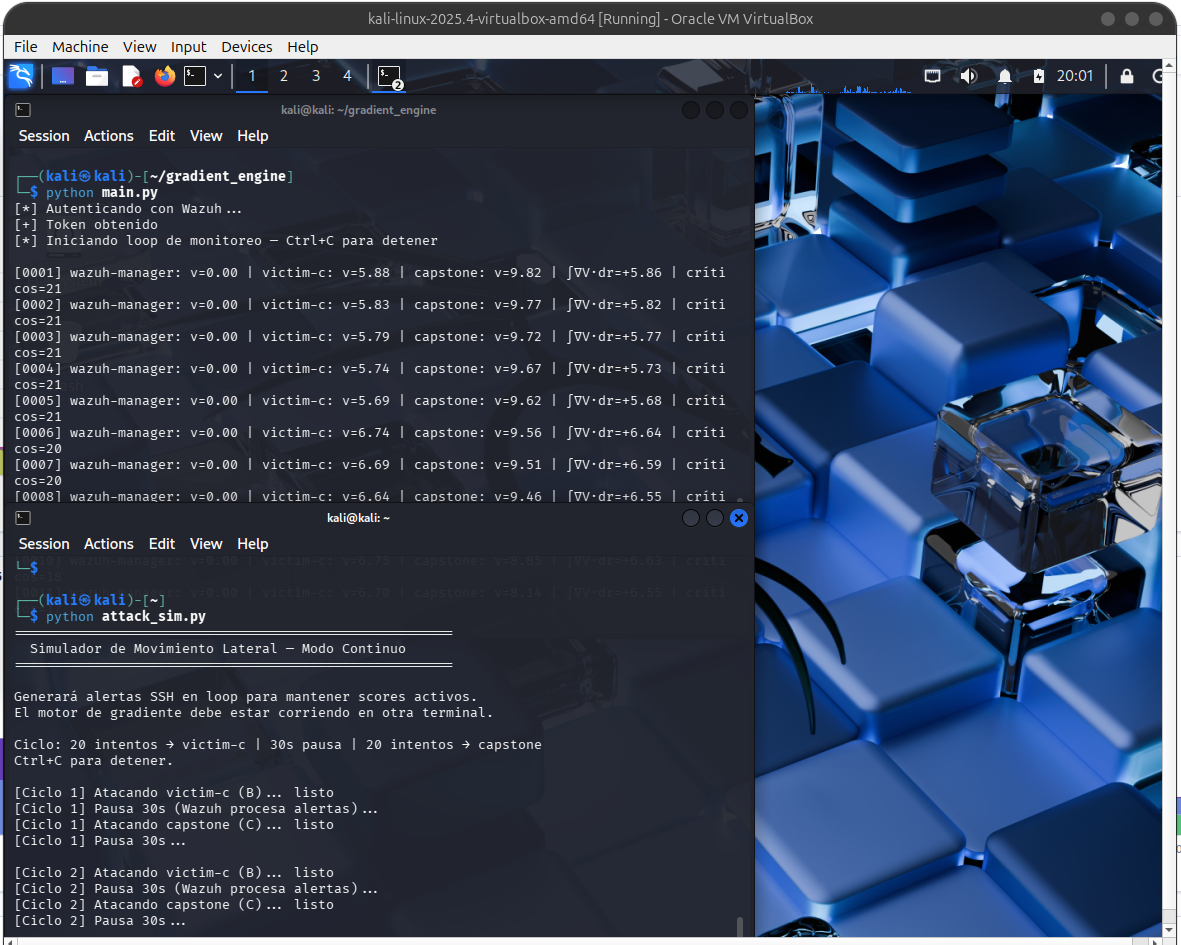
\includegraphics[width=0.85\linewidth]{kali_attack_sim}
  \caption{Terminal de Kali con \texttt{attack\_sim.py} en ejecución.
    Se observan los ciclos de ataque: 20 intentos hacia victim-c,
    pausa de 30\,s para procesamiento de Wazuh, y 20 intentos hacia
    capstone. El contador de ciclos indica que el simulador ya lleva
    varios minutos activo.}
  \label{fig:kali_attack_sim}
\end{figure}

\subsection{Motor en tiempo real}

\begin{figure}[H]
  \centering
  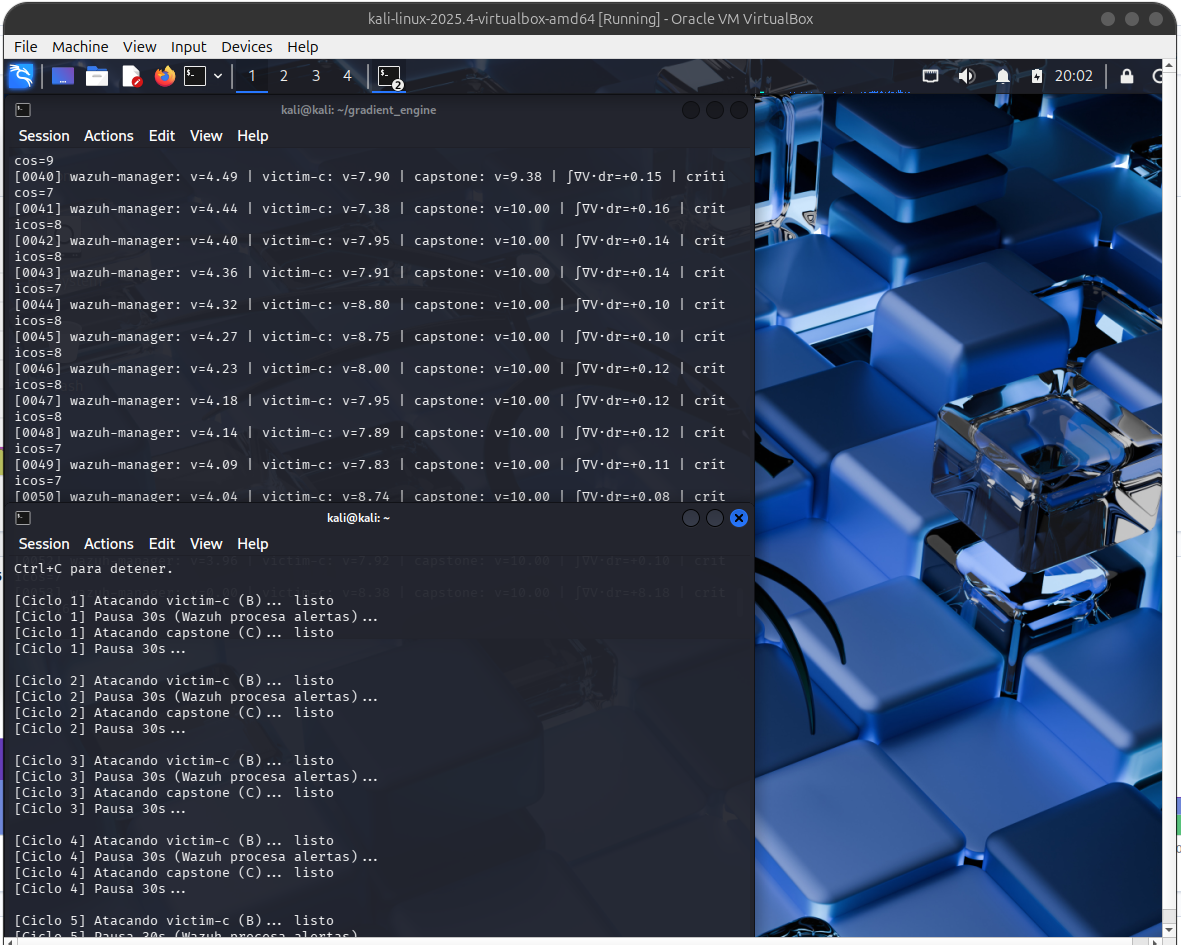
\includegraphics[width=0.85\linewidth]{kali_gradient_engine}
  \caption{Terminal de Kali con \texttt{main.py} mostrando la salida
    por consola del motor de gradiente. Cada línea corresponde a una
    iteración e incluye: número de iteración, score de cada nodo
    ($v_A$, $v_B$, $v_C$) e integral de línea $\int\grad V\cdot d\mathbf{r}$.
    Se aprecia cómo los scores de victim-c y capstone crecen a medida
    que las alertas SSH se registran en Wazuh.}
  \label{fig:kali_engine}
\end{figure}

\subsection{Alertas registradas en Wazuh --- victim-c}

\begin{figure}[H]
  \centering
  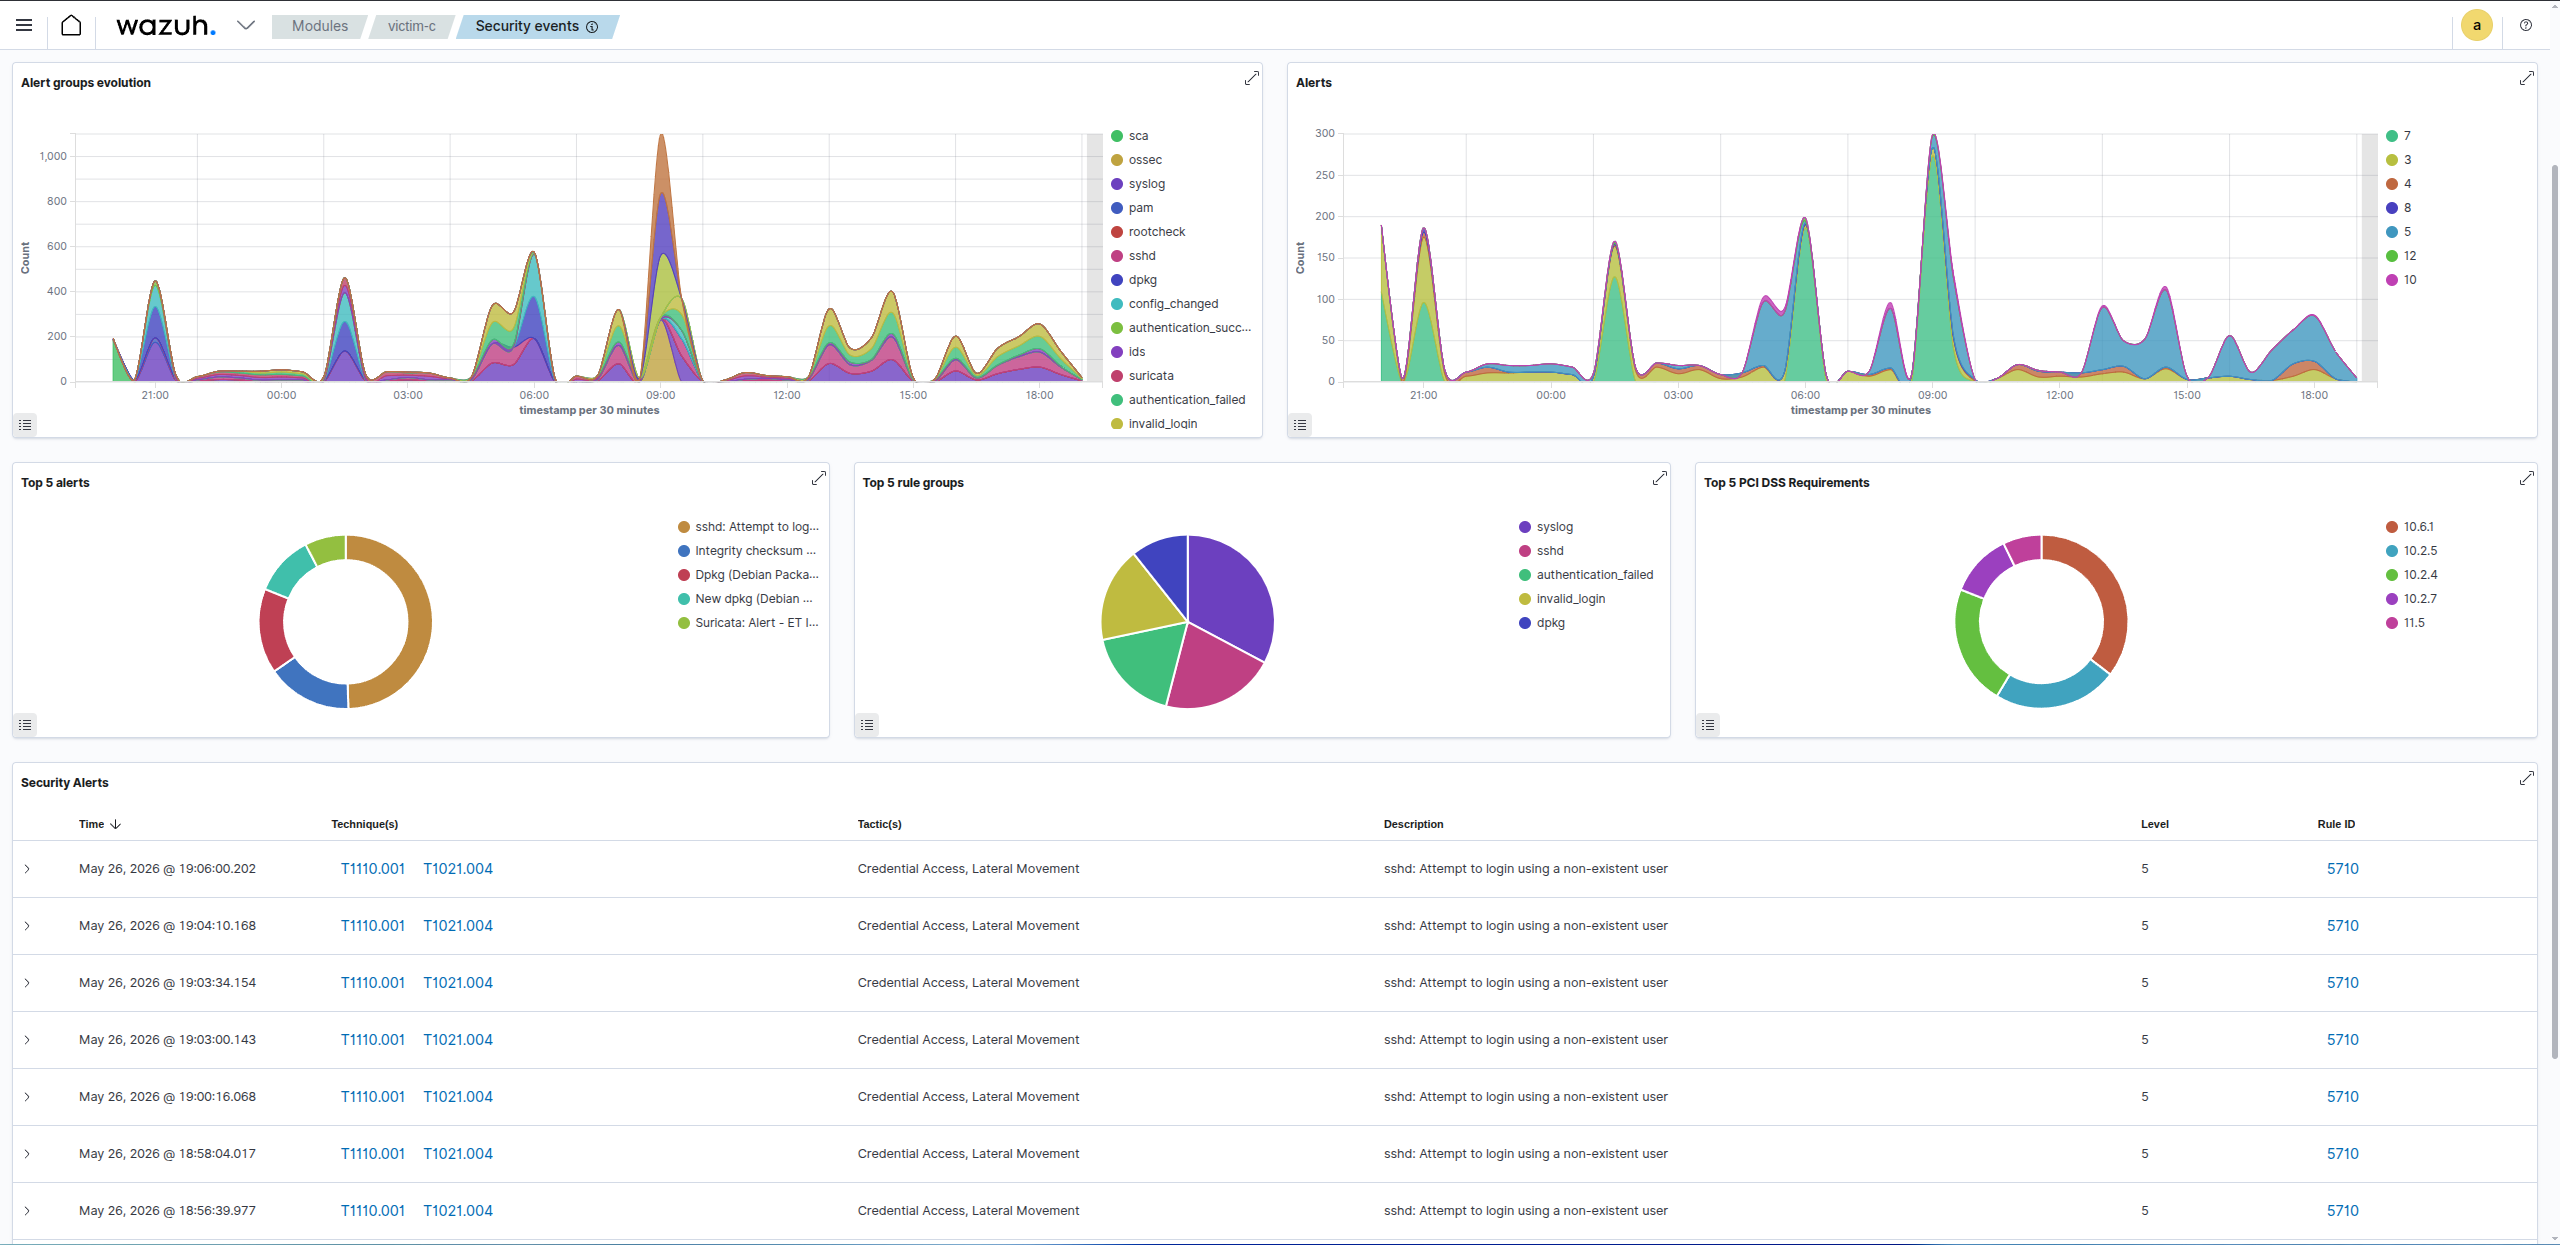
\includegraphics[width=\linewidth]{wazuh_events_victimc}
  \caption{Security Events de Wazuh filtrado a victim-c (agent~003).
    \textit{Arriba izquierda}: evolución de grupos de alertas en las
    últimas 24\,h --- el pico de \texttt{sshd} y
    \texttt{authentication\_failed} coincide con la sesión de laboratorio.
    \textit{Abajo}: lista de alertas en tiempo real; todas clasificadas
    como T1110.001 + T1021.004 (\emph{Credential Access, Lateral
    Movement}), nivel~5, Rule~5710 (\emph{sshd: Attempt to login using
    a non-existent user}).}
  \label{fig:wazuh_victimc}
\end{figure}

\subsection{Clasificación MITRE ATT\&CK}

\textbf{MITRE ATT\&CK} (\emph{Adversarial Tactics, Techniques and
Common Knowledge}) es un marco de referencia global que cataloga
tácticas y técnicas usadas por atacantes reales, organizadas en una
matriz. Wazuh enriquece automáticamente cada alerta con la táctica y
técnica MITRE correspondiente, permitiendo clasificar el ataque en
términos estándar de la industria. Las relevantes para este experimento
son:
\begin{itemize}
  \item \textbf{TA0008 --- Lateral Movement}: táctica que describe el
    movimiento de un adversario por los sistemas de una red comprometida.
  \item \textbf{T1110.001 --- Brute Force: Password Guessing}: técnica
    de intentar credenciales comunes para autenticarse.
  \item \textbf{T1021.004 --- Remote Services: SSH}: acceso remoto a
    sistemas mediante el protocolo SSH.
\end{itemize}

\begin{figure}[H]
  \centering
  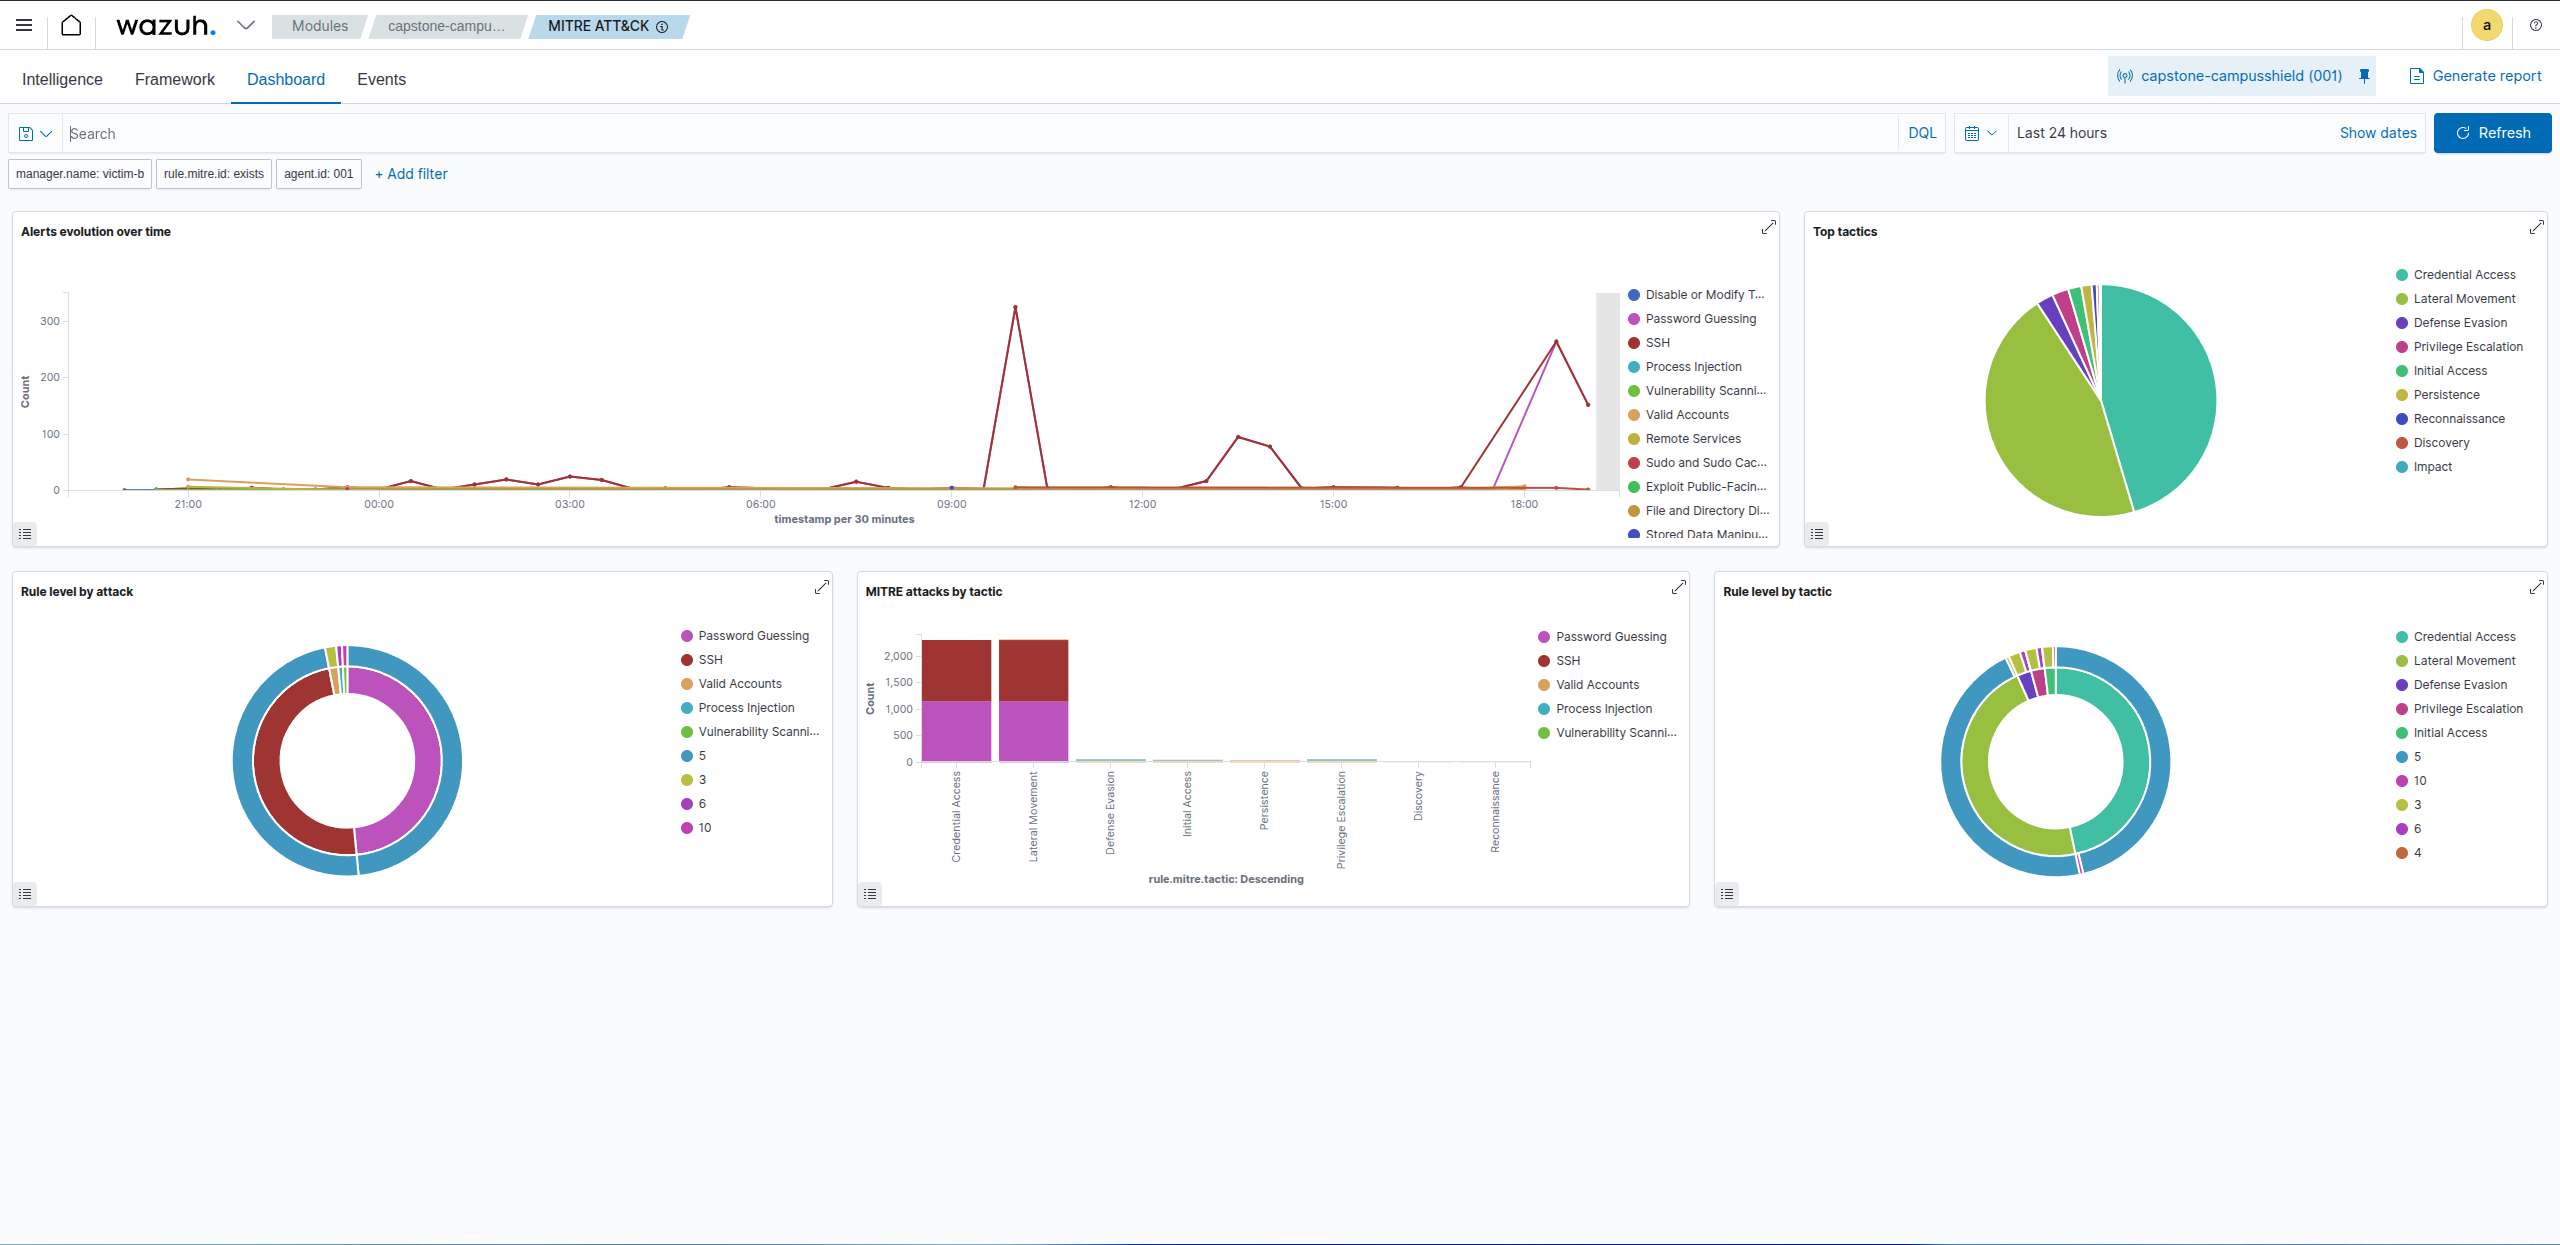
\includegraphics[width=\linewidth]{mitre_dashboard}
  \caption{Dashboard MITRE ATT\&CK de Wazuh para capstone
    (agent~001, filtrado a las últimas 24\,h). Las tácticas dominantes
    son \textbf{Credential Access} y \textbf{Lateral Movement}, con
    aproximadamente 2\,000 eventos cada una en el gráfico de barras
    central. El pie chart de la derecha confirma que SSH y
    \emph{Password Guessing} concentran la mayoría de las técnicas
    detectadas, alineándose con los ataques brute-force del simulador.}
  \label{fig:mitre_dashboard}
\end{figure}

% ═════════════════════════════════════════════════════════════════════════════
\section{Resultados y análisis}

\subsection{Evolución del campo escalar durante el experimento}

Las figuras~\ref{fig:motor_iter1}, \ref{fig:motor_iter37}
y~\ref{fig:motor_iter53} muestran el estado del motor en tres momentos
representativos: inicio del experimento, fase estable y estado final.
Cada figura contiene tres paneles: campo escalar $V$, gradiente
$\grad V$, y trayectoria $\mathbf{r}(t)$.

\begin{figure}[H]
  \centering
  \includegraphics[width=\linewidth]{gradient_fig_0001}
  \caption{\textbf{Iteración 1.} Los nodos B (victim-c, $v=5.88$) y C
    (capstone, $v=9.82$) ya muestran picos activos porque el simulador
    comenzó antes de esta captura. \textit{Panel izquierdo}: dos
    gaussianas bien diferenciadas con capstone claramente más intensa.
    \textit{Panel central}: el campo $\grad V$ muestra flechas que
    convergen hacia ambos picos; se aprecia la región de silla entre
    B y C donde las flechas se «abren» en direcciones opuestas.
    \textit{Panel derecho}: la trayectoria en etapa A$\to$B (azul)
    parte del punto de entrada $(0.5, 0.5)$ y converge hacia victim-c.
    Integral de línea: $+5.86$. Puntos críticos detectados: 21.}
  \label{fig:motor_iter1}
\end{figure}

\begin{figure}[H]
  \centering
  \includegraphics[width=\linewidth]{gradient_fig_0037}
  \caption{\textbf{Iteración 37.} Estado estable del experimento.
    Scores: $v_B = 8.23$, $v_C = 9.89$. Los dos picos gaussianos están
    bien desarrollados y la región de silla entre ellos es claramente
    visible en el panel de gradiente como zona de baja magnitud vectorial
    (flechas más cortas). La trayectoria A$\to$B (azul) y B$\to$C
    (naranja punteado) muestra el patrón completo de movimiento lateral.
    Integral de línea: $+8.04$.}
  \label{fig:motor_iter37}
\end{figure}

\begin{figure}[H]
  \centering
  \includegraphics[width=\linewidth]{gradient_fig_0053}
  \caption{\textbf{Iteración 53 (estado final).} Capstone alcanza su
    score máximo ($v_C = 10.0$, saturado), mientras victim-c mantiene
    $v_B = 8.38$. El campo V muestra dos picos prácticamente iguales
    en intensidad con la silla bien definida. La integral de línea
    $+8.18$ es la más alta registrada en el experimento. Puntos
    críticos: 16.}
  \label{fig:motor_iter53}
\end{figure}

\subsection{Observación 1 --- $V$ responde en tiempo real}

A medida que el simulador enviaba intentos SSH, los scores crecieron
proporcionalmente al volumen de alertas recibidas:

\begin{table}[H]
  \centering
  \caption{Evolución de scores e integral de línea durante el experimento.}
  \begin{tabular}{@{}ccccc@{}}
    \toprule
    Iteración & $v_A$ & $v_B$ & $v_C$ & $\int\grad V\cdot d\mathbf{r}$ \\
    \midrule
    1  & 0.00 &  5.88 &  9.82 & $+5.86$ \\
    9  & 0.00 &  7.39 &  8.90 & $+7.22$ \\
    37 & 0.00 &  8.23 &  9.89 & $+8.04$ \\
    53 & 0.00 &  8.38 & 10.00 & $+8.18$ \\
    \bottomrule
  \end{tabular}
\end{table}

La integral creció de forma monotónica con los scores, validando
empíricamente el Teorema Fundamental de Integrales de Línea:
$\int\grad V\cdot d\mathbf{r} = V(\text{destino}) - V(\text{origen})$.

\subsection{Observación 2 --- El saddle point es el hallazgo topológico central}

En todas las figuras con dos nodos activos, el panel de gradiente muestra
una región donde las flechas se «abren» en dos conjuntos opuestos.
Esa región corresponde a un \textbf{punto de silla} del campo escalar:
un punto crítico donde el Hessiano tiene eigenvalores de signo opuesto.
Matemáticamente separa las dos cuencas de atracción del campo.

\begin{tcolorbox}[defbox]
  \textbf{Implicación defensiva.} El saddle point ($\approx (5,3)$
  entre B y C) es el cuello de botella topológico de la red. Colocar
  controles de acceso o honeypots en esa zona maximiza la probabilidad
  de interceptar al atacante en tránsito entre los dos nodos.
\end{tcolorbox}

\subsection{Observación 3 --- Puntos críticos correlacionan con estructura del campo}

\begin{table}[H]
  \centering
  \caption{Puntos críticos detectados según el estado del campo.}
  \begin{tabular}{@{}lcc@{}}
    \toprule
    Estado del campo & Puntos críticos & Interpretación \\
    \midrule
    1 nodo activo   & 46--94 & Campo casi plano fuera del pico --- artefactos \\
    2 nodos activos & 13--21 & Campo bien estructurado con silla definida \\
    3 nodos activos & 5--8   & Estructura muy clara, mínimos y máximos separados \\
    \bottomrule
  \end{tabular}
\end{table}

\subsection{Observación 4 --- Tres nodos activos colapsan la integral}

En las iteraciones 23--35, el wazuh-manager generó alertas propias
($v_A \approx 4$). El pico gaussiano de A «empuja» al atacante de
vuelta desde el punto de entrada, haciendo que la integral caiga a
valores $\approx 0.07$--$0.13$:

\begin{table}[H]
  \centering
  \caption{Iteraciones con nodo A activo.}
  \begin{tabular}{@{}ccccc@{}}
    \toprule
    Iter & $v_A$ & $v_B$ & $v_C$ & $\int\grad V\cdot d\mathbf{r}$ \\
    \midrule
    26 & 4.41 & 8.10 &  8.03 & $+0.13$ \\
    33 & 4.09 & 9.04 &  9.56 & $+0.07$ \\
    35 & 4.01 & 8.33 & 10.00 & $+0.09$ \\
    \bottomrule
  \end{tabular}
\end{table}

Esto es una limitación identificada del modelo: en producción
se requeriría filtrar por tipo de alerta para excluir ruido operacional
del nodo de entrada.

\subsection{Observación 5 --- La trayectoria A$\to$B$\to$C valida el movimiento lateral}

La integración en dos etapas reproduce el patrón clásico de movimiento
lateral de MITRE TA0008:
\begin{itemize}
  \item \textbf{Etapa A$\to$B} (azul): el flujo gradiente desde
    $(0.5,0.5)$ converge hacia victim-c, el primer máximo local
    accesible. Replica la fase de «pivote inicial».
  \item \textbf{Etapa B$\to$C} (naranja): desde el pivote en B, el
    flujo reanuda hacia capstone. Una vez comprometido B, el gradiente
    orienta al atacante hacia el activo de mayor valor.
\end{itemize}

% ═════════════════════════════════════════════════════════════════════════════
\section{Discusión: alcances, limitaciones y posibles mejoras}

\subsection{Alcances}

\begin{itemize}
  \item $V(x,y)$ convierte la noción abstracta de «vulnerabilidad»
    en un campo escalar operable con herramientas de cálculo vectorial
  \item $\grad V$ formaliza la dirección óptima del ataque en cada punto
  \item $\mathbf{r}(t)$ describe la trayectoria como curva parametrizada
    con solución analítica exacta en la Fase~1
  \item La integral de línea cuantifica la exposición acumulada
    independientemente de la ruta (conservatividad verificada)
  \item El experimento con datos reales de Wazuh confirma que el campo
    responde de forma coherente a los ataques simulados
\end{itemize}

\subsection{Limitaciones}

\textbf{Modelo analítico (Fase~1):} la función $V$ fue diseñada para
satisfacer las propiedades matemáticas deseadas, no derivada de datos
empíricos. Una red real es un grafo discreto con firewalls, credenciales
y segmentos; el plano continuo es una idealización.

\textbf{Modelo dinámico (Fase~2):}
\begin{itemize}
  \item El score basado en niveles de alerta puede ser ruidoso: alertas
    operacionales del nodo de entrada distorsionan el campo
  \item El parámetro $\sigma$ requiere calibración empírica por red
  \item La interpolación gaussiana no respeta la topología real
\end{itemize}

\subsection{Posibles mejoras}

\begin{itemize}
  \item \textbf{Grafo discreto ponderado}: reemplazar el plano continuo
    por un grafo con aristas ponderadas por dificultad de movimiento
  \item \textbf{Superficie 3D}: modelar $z = V(x,y)$ para visualizar
    el «relieve de vulnerabilidad» de la red
  \item \textbf{Barreras defensivas}: incorporar firewalls y MFA como
    barreras de potencial donde $V$ tiene una discontinuidad
  \item \textbf{Integración con OpenCTI}: usar TTPs de MITRE ATT\&CK
    para asignar pesos fundamentados por técnica de ataque
\end{itemize}

% ═════════════════════════════════════════════════════════════════════════════
\section{Bitácora de uso de inteligencia artificial}

\subsection*{Herramienta utilizada}

Se utilizó \textbf{Claude} (Anthropic) como asistente de inteligencia
artificial a lo largo del proyecto, principalmente en dos roles:
generación de código Python y contraste conceptual para definir el
enfoque del modelo.

\subsection*{Generación de código}

El motor de gradiente completo (\texttt{wazuh\_client.py},
\texttt{scalar\_field.py}, \texttt{gradient\_flow.py},
\texttt{visualizer.py}, \texttt{main.py} y \texttt{attack\_sim.py})
fue desarrollado en colaboración con Claude. El proceso consistió en
describir el objetivo de cada módulo, revisar el código generado,
identificar errores de ejecución y solicitar correcciones iterativas.
Claude no tomó decisiones de diseño de forma autónoma: cada elección
(uso de RK45, normalización logarítmica, integración en dos etapas,
acceso vía SSH al archivo de alertas) fue discutida y validada antes
de implementarse.

\subsection*{Definición del enfoque y campo de aplicación}

La idea central de modelar el movimiento lateral como flujo gradiente
surgió de contrastar conocimientos propios de la carrera de ingeniería
y de certificaciones de ciberseguridad (familiaridad con el marco
MITRE ATT\&CK, con la arquitectura de SIEMs y con la etapa de
movimiento lateral en ataques APT) con las sugerencias de Claude sobre
cómo representar matemáticamente ese fenómeno usando cálculo vectorial.

La sesión de trabajo con Claude funcionó como un diálogo técnico: el
estudiante aportó el contexto de dominio (qué es un agente Wazuh, cómo
se generan alertas SSH, qué significa una táctica MITRE) y Claude
aportó la formalización matemática (cómo construir $V$ como
superposición gaussiana, cómo expresar la trayectoria como solución de
una EDO, cómo verificar conservatividad). El enfoque final — campo
escalar de vulnerabilidad con decaimiento temporal, flujo gradiente
como trayectoria del atacante, saddle point como cuello de botella
defensivo — es producto de ese contraste iterativo.

\subsection*{Reutilización del laboratorio}

La infraestructura de DigitalOcean (manager Wazuh, victim-c y
capstone-campusshield) fue reutilizada de un laboratorio de
\textbf{Cyber Threat Intelligence (CTI)} desarrollado previamente en
otra asignatura. Dicho laboratorio ya tenía los agentes Wazuh
instalados y configurados, Suricata activo con reglas Emerging Threats,
y conectividad entre nodos. Para este proyecto se adaptó la
infraestructura existente habilitando autenticación por contraseña en
capstone y desarrollando el motor de gradiente como capa de análisis
sobre los datos de alertas ya disponibles.

\subsection*{Lo que la IA no hizo}

Claude no definió el fenómeno de interés, no eligió el campo de
aplicación ni determinó qué conceptos de cálculo vectorial eran
pertinentes. Tampoco ejecutó el laboratorio ni interpretó los
resultados: la lectura de los scores, la identificación del saddle
point y las conclusiones defensivas son producto del análisis propio
contrastado con el modelo generado.

% ═════════════════════════════════════════════════════════════════════════════
\section{Conclusiones}

El proyecto demuestra que el cálculo vectorial puede aplicarse de forma
rigurosa a un fenómeno de ciberseguridad. El movimiento lateral de un
atacante tiene una estructura matemática precisa: un campo escalar de
vulnerabilidad $V$ cuyo gradiente $\grad V$ orienta la trayectoria
hacia los activos de mayor exposición.

Los siete conceptos del curso utilizados cumplen cada uno una función
interpretativa concreta dentro del modelo:

\begin{itemize}
  \item El \textbf{gradiente} formalizó la dirección óptima del ataque
  \item La \textbf{curva parametrizada} $\mathbf{r}(t) = \bigl(7.4(1-e^{-2t}),\;
    3.25(1-e^{-2t})\bigr)$ describió analíticamente el recorrido
  \item La \textbf{integral de línea} ($= 65.1$) cuantificó la exposición
    acumulada independientemente de la ruta
  \item La \textbf{conservatividad} reveló que solo importan el origen
    y el destino, no el camino
  \item El \textbf{punto crítico} con Hessiana negativa definida
    identificó matemáticamente la zona de mayor vulnerabilidad
  \item El \textbf{punto de silla} entre B y C emergió como el cuello
    de botella topológico donde concentrar las defensas
  \item La \textbf{irrotacionalidad} confirmó que no existen bucles
    de vulnerabilidad cerrados en el modelo
\end{itemize}

La extensión al laboratorio con Wazuh y Suricata convierte el modelo
teórico en un experimento verificable. Los datos reales confirman que
el campo $V$ responde coherentemente al volumen de alertas, la trayectoria
A$\to$B$\to$C es reproducible, y el saddle point entre nodos es un
hallazgo topológico con implicaciones defensivas concretas.

Defender la red significa \textbf{reducir las pendientes del campo
$\grad V$} que conducen hacia los activos críticos: una idea que el
cálculo vectorial hace precisa y cuantificable.

% ═════════════════════════════════════════════════════════════════════════════
\section{Referencias bibliográficas}

\begin{enumerate}[label={[\arabic*]}]
  \item Marsden, J.~E., \& Tromba, A. (2012). \textit{Vector Calculus}
    (6th ed.). W.\,H.\ Freeman.
  \item MITRE ATT\&CK. \textit{Lateral Movement, Tactic TA0008}.
    \url{https://attack.mitre.org/tactics/TA0008/}
  \item MITRE ATT\&CK. \textit{T1110.001 --- Brute Force: Password Guessing}.
    \url{https://attack.mitre.org/techniques/T1110/001/}
  \item MITRE ATT\&CK. \textit{T1021.004 --- Remote Services: SSH}.
    \url{https://attack.mitre.org/techniques/T1021/004/}
  \item Wazuh. \textit{Wazuh Documentation v4.7}.
    \url{https://documentation.wazuh.com/current/}
  \item Suricata. \textit{Suricata User Guide}.
    \url{https://docs.suricata.io/}
  \item CISA. \textit{StopRansomware Guide}.
    \url{https://www.cisa.gov/stopransomware/ransomware-guide}
\end{enumerate}

% ═════════════════════════════════════════════════════════════════════════════
\newpage
\section*{Anexos: Evidencia fotográfica complementaria}
\addcontentsline{toc}{section}{Anexos: Evidencia fotográfica complementaria}

Las siguientes capturas complementan la evidencia presentada en el
cuerpo del informe. Se incluyen para completitud del registro pero
no son estrictamente necesarias para seguir el argumento principal.

\subsection*{A.1 Dashboard global de Security Events}

\begin{figure}[H]
  \centering
  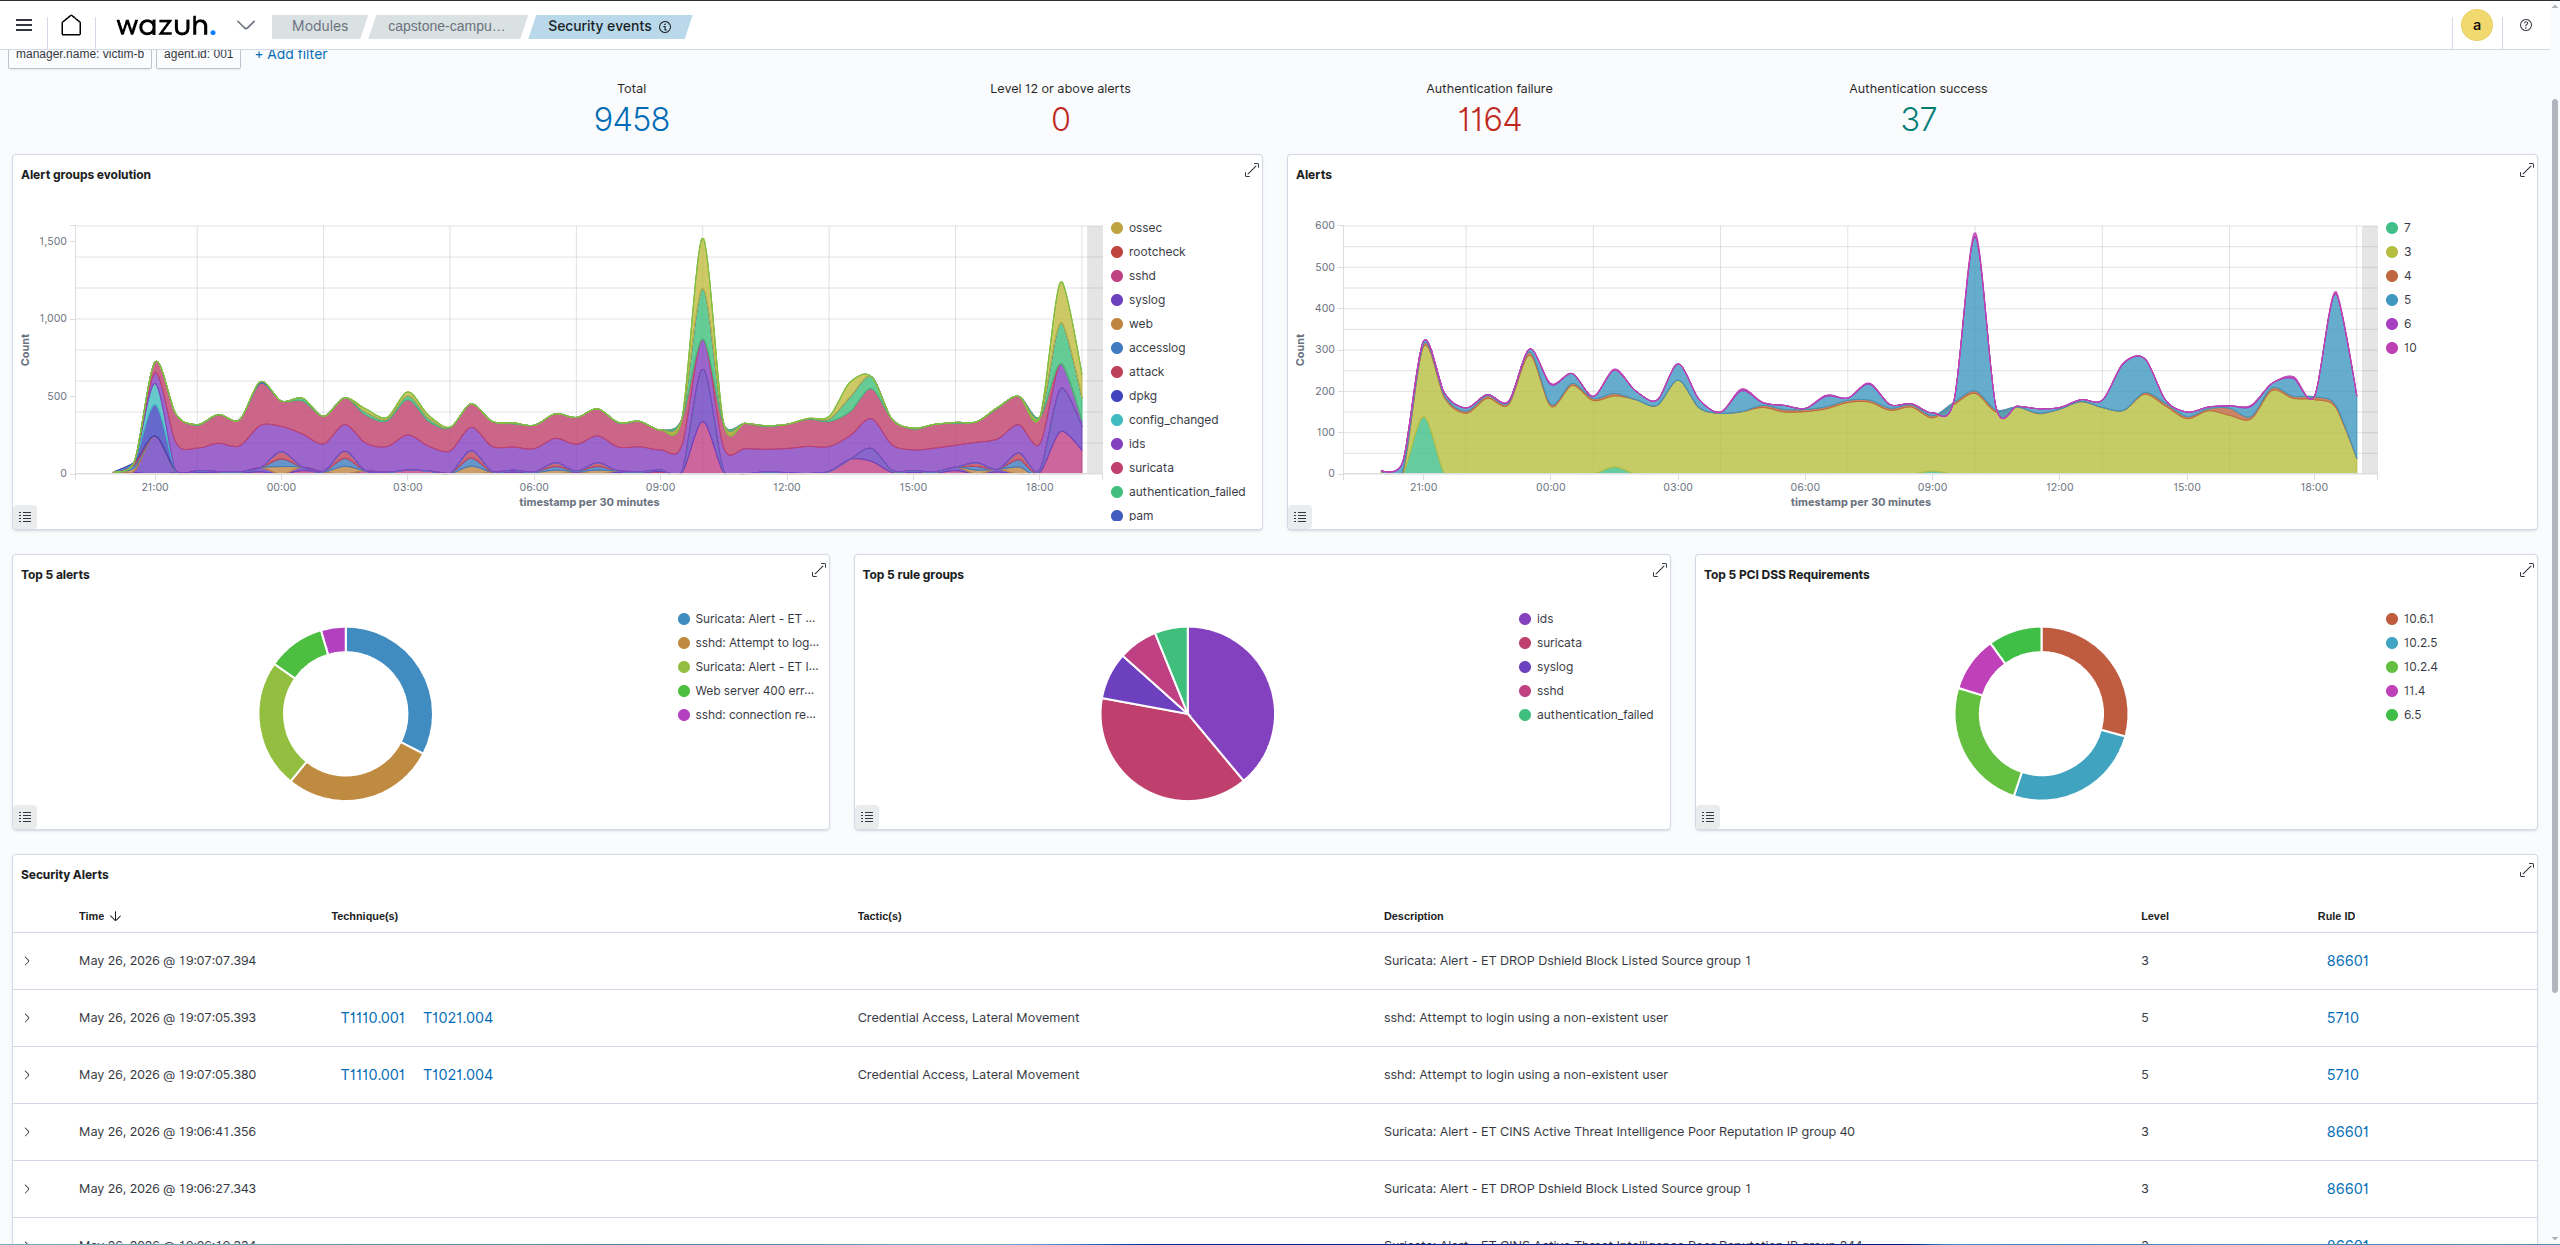
\includegraphics[width=\linewidth]{wazuh_events_capstone}
  \caption{Security Events de capstone-campusshield (agent~001):
    9\,458 alertas totales, \textbf{1\,164 fallos de autenticación}
    y 37 éxitos en las últimas 24\,h. Se distinguen alertas Suricata
    (ET DROP, CINS) y alertas sshd. Los fallos de autenticación son
    las alertas que el motor consume para calcular el score de capstone.}
\end{figure}

\subsection*{A.2 Eventos MITRE detallados}

\begin{figure}[H]
  \centering
  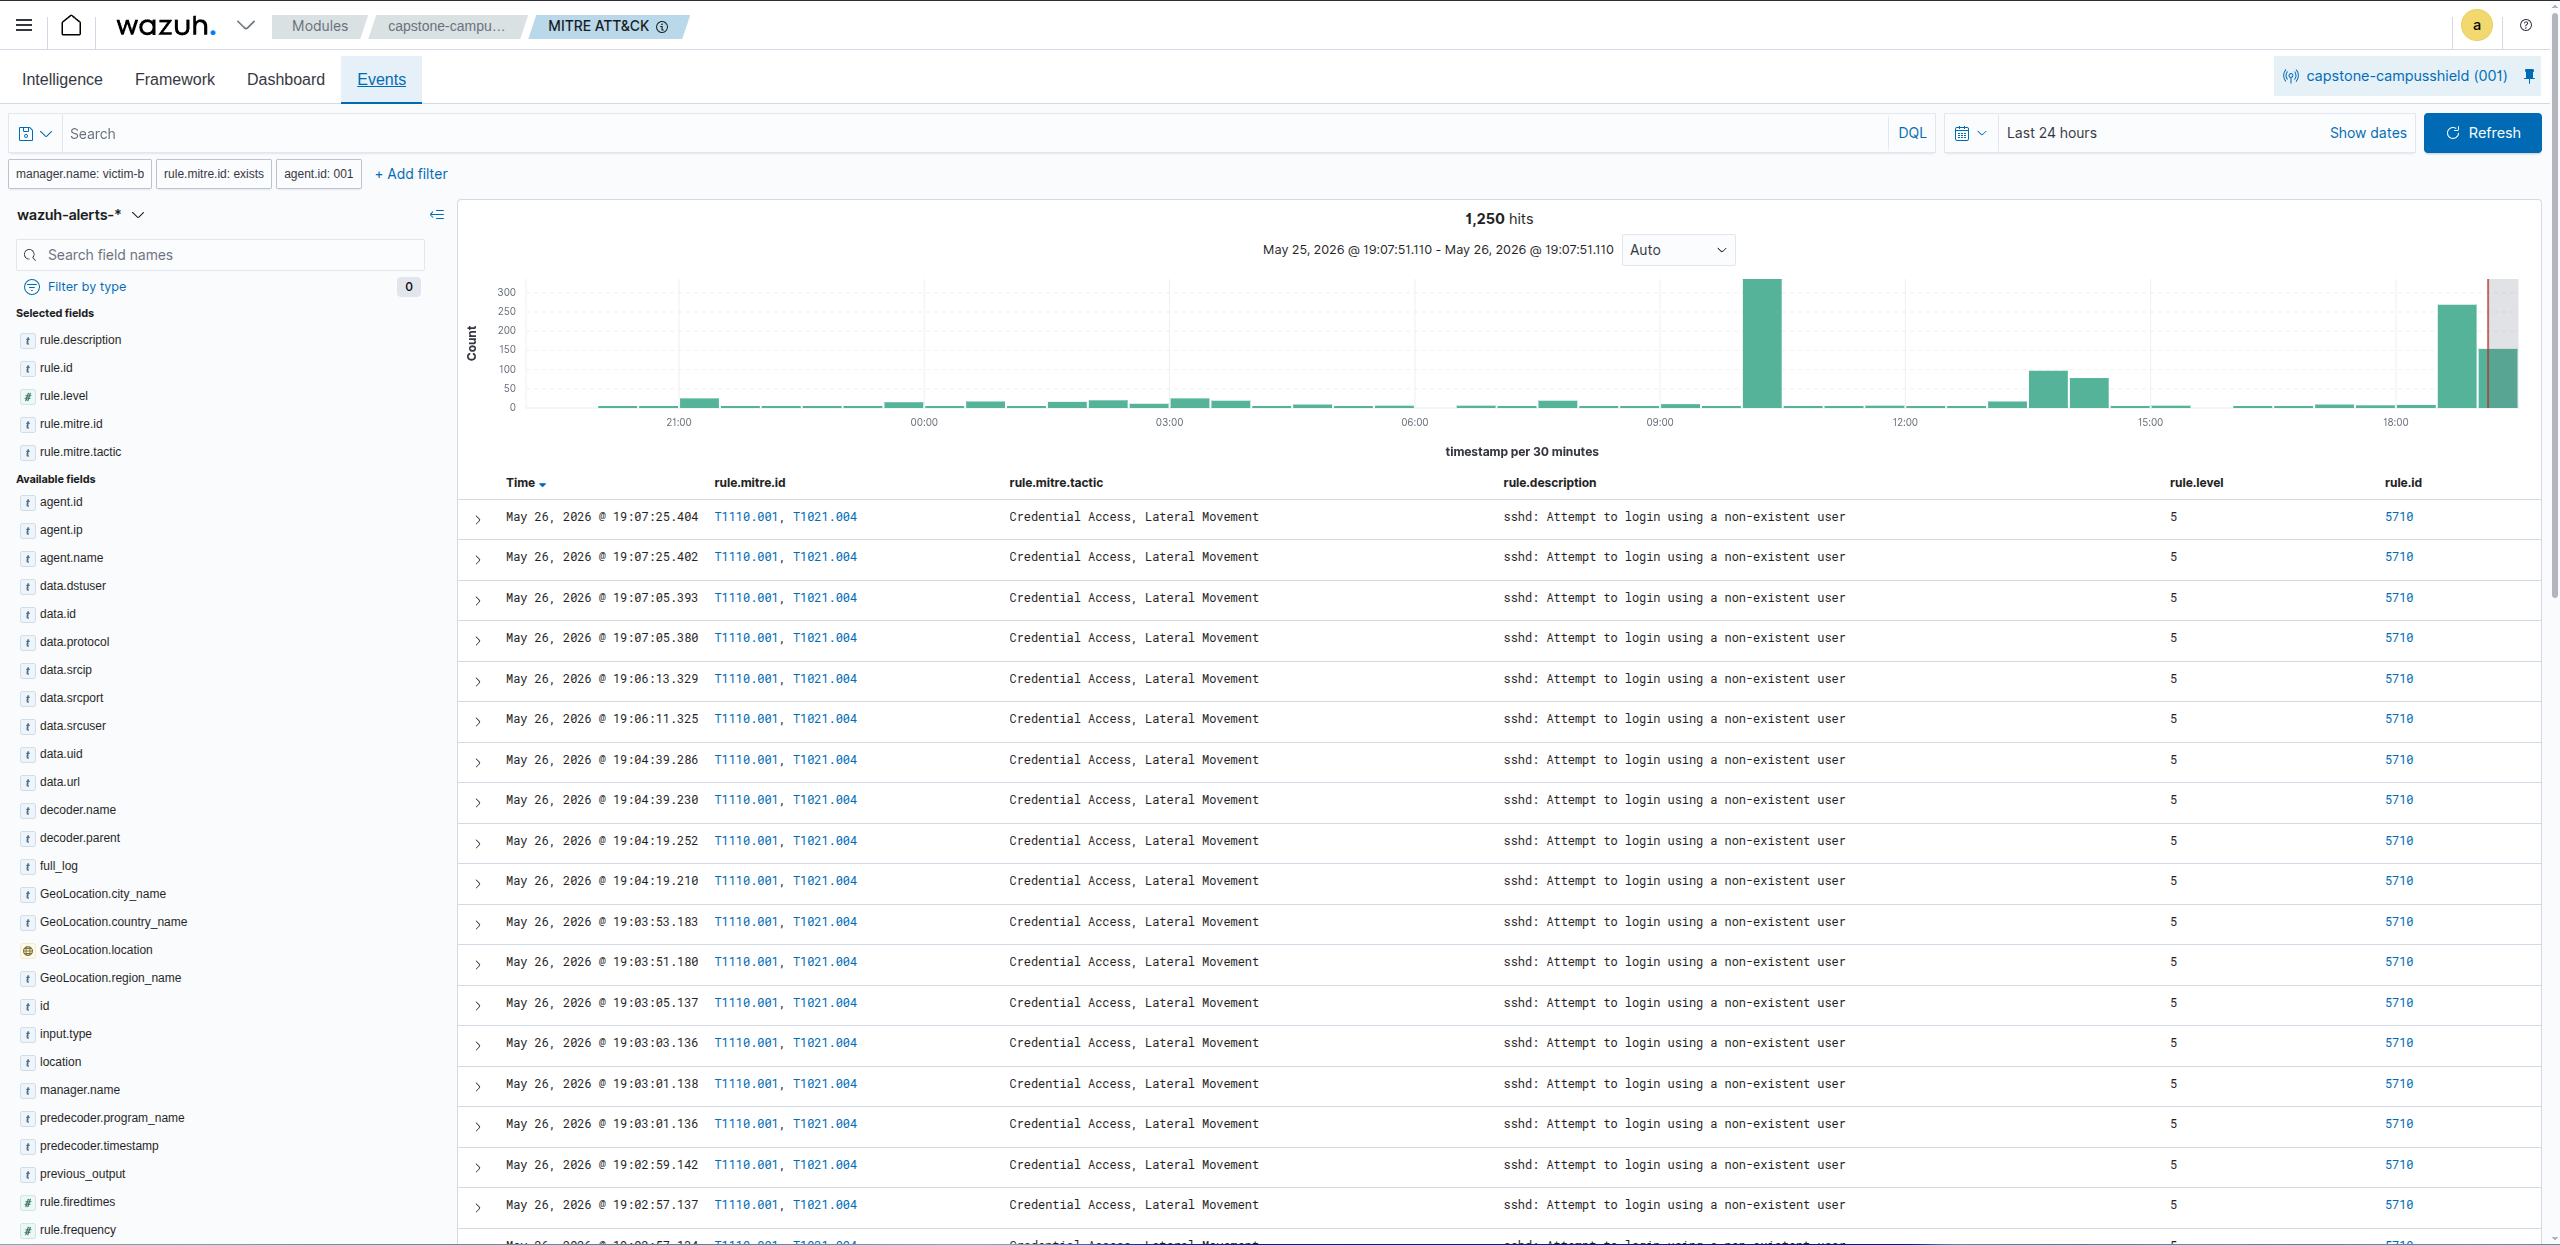
\includegraphics[width=\linewidth]{mitre_events}
  \caption{Vista de eventos MITRE ATT\&CK para capstone:
    1\,250 hits en 24\,h, todos clasificados como T1110.001 +
    T1021.004 (\emph{Credential Access + Lateral Movement}),
    nivel~5, Rule~5710. La vista confirma que la totalidad de los
    eventos provienen de intentos SSH con usuarios inexistentes,
    generados por el simulador \texttt{attack\_sim.py}.}
\end{figure}

\subsection*{A.3 Integrity Monitoring}

\begin{figure}[H]
  \centering
  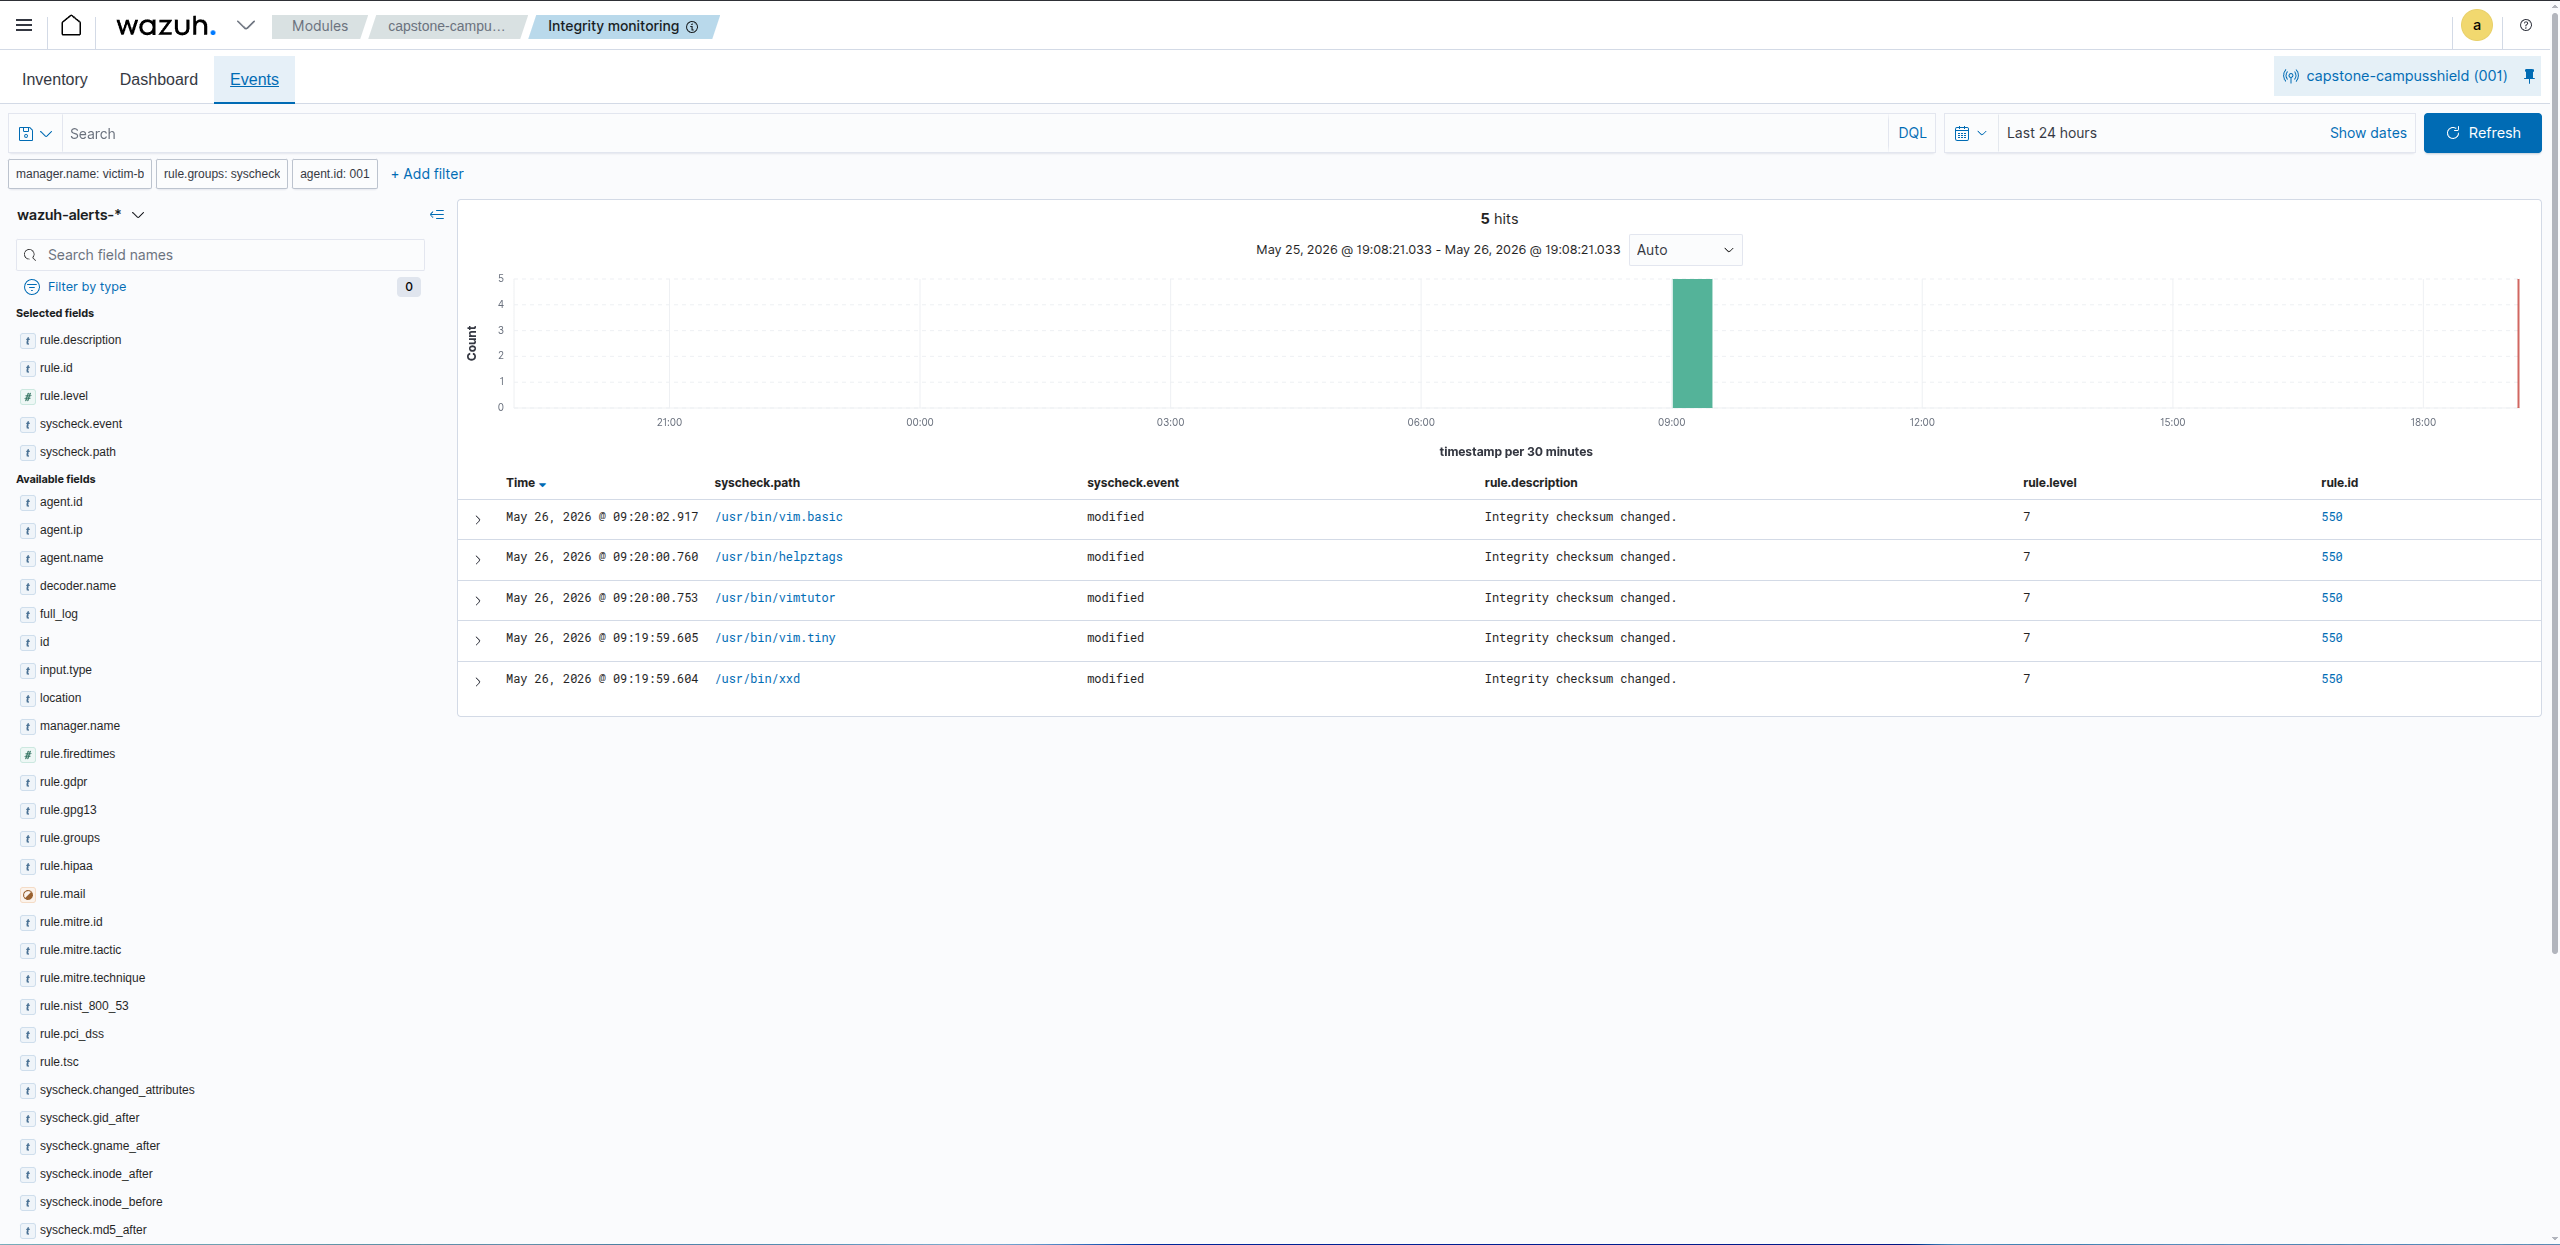
\includegraphics[width=\linewidth]{wazuh_fim}
  \caption{Integrity Monitoring (FIM) de capstone: 5 modificaciones
    detectadas en binarios del sistema (\texttt{/usr/bin/vim.basic},
    \texttt{/usr/bin/helpztags}, \texttt{/usr/bin/vimtutor},
    \texttt{/usr/bin/vim.tiny}, \texttt{/usr/bin/xxd}), Rule~550
    \emph{Integrity checksum changed}, nivel~7. Estas modificaciones
    corresponden a una actualización de paquetes en el nodo y no a
    actividad del atacante; sin embargo, ilustran la capacidad del
    agente Wazuh para detectar cambios en el sistema de archivos.}
\end{figure}

\end{document}
